% !TEX TS-program = XeLaTeX
% use the following command:
% all document files must be coded in UTF-8
\documentclass[english]{textolivre}
% build HTML with: make4ht -e build.lua -c textolivre.cfg -x -u article "fn-in,svg,pic-align"

\journalname{Texto Livre}
\thevolume{15}
%\thenumber{1} % old template
\theyear{2022}
\receiveddate{\DTMdisplaydate{2022}{5}{1}{-1}} % YYYY MM DD
\accepteddate{\DTMdisplaydate{2022}{6}{1}{-1}}
\publisheddate{\DTMdisplaydate{2022}{8}{14}{-1}}
\corrauthor{Amina Tahraoui}
\articledoi{10.35699/1983-3652.2022.39545}
%\articleid{NNNN} % if the article ID is not the last 5 numbers of its DOI, provide it using \articleid{} commmand 
% list of available sesscions in the journal: articles, dossier, reports, essays, reviews, interviews, editorial
\articlesessionname{articles}
\runningauthor{Tahraoui} 
%\editorname{Leonardo Araújo} % old template
\sectioneditorname{Daniervelin Pereira}
\layouteditorname{Leonado Araújo}

\title{Teaching sight and bilateral interpreting online: students’ perceptions of teacher feedback}
\othertitle{Ensino de visão e interpretação bilateral \textit{online}: percepções dos alunos sobre o \textit{feedback} do professor}
% if there is a third language title, add here:
%\othertitle{Artikelvorlage zur Einreichung beim Texto Livre Journal}

\author[1]{Amina Tahraoui \orcid{0000-0002-4214-987X} \thanks{Email: \href{mailto:atahraoui@pnu.edu.sa}{atahraoui@pnu.edu.sa}}}
\affil[1]{Princess Nourah bint Abdulrahman University, College of Languages, Translation Department, Riyadh, Saudi Arabia.}

\addbibresource{article.bib}
% use biber instead of bibtex
% $ biber article

% used to create dummy text for the template file
\definecolor{dark-gray}{gray}{0.35} % color used to display dummy texts
\usepackage{lipsum}
\SetLipsumParListSurrounders{\colorlet{oldcolor}{.}\color{dark-gray}}{\color{oldcolor}}

% used here only to provide the XeLaTeX and BibTeX logos
\usepackage{hologo}

% if you use multirows in a table, include the multirow package
\usepackage{multirow}

% provides sidewaysfigure environment
\usepackage{rotating}

% CUSTOM EPIGRAPH - BEGIN 
%%% https://tex.stackexchange.com/questions/193178/specific-epigraph-style
\usepackage{epigraph}
\renewcommand\textflush{flushright}
\makeatletter
\newlength\epitextskip
\pretocmd{\@epitext}{\em}{}{}
\apptocmd{\@epitext}{\em}{}{}
\patchcmd{\epigraph}{\@epitext{#1}\\}{\@epitext{#1}\\[\epitextskip]}{}{}
\makeatother
\setlength\epigraphrule{0pt}
\setlength\epitextskip{0.5ex}
\setlength\epigraphwidth{.7\textwidth}
% CUSTOM EPIGRAPH - END

% LANGUAGE - BEGIN
% ARABIC
% for languages that use special fonts, you must provide the typeface that will be used
% \setotherlanguage{arabic}
% \newfontfamily\arabicfont[Script=Arabic]{Amiri}
% \newfontfamily\arabicfontsf[Script=Arabic]{Amiri}
% \newfontfamily\arabicfonttt[Script=Arabic]{Amiri}
%
% in the article, to add arabic text use: \textlang{arabic}{ ... }
%
% RUSSIAN
% for russian text we also need to define fonts with support for Cyrillic script
% \usepackage{fontspec}
% \setotherlanguage{russian}
% \newfontfamily\cyrillicfont{Times New Roman}
% \newfontfamily\cyrillicfontsf{Times New Roman}[Script=Cyrillic]
% \newfontfamily\cyrillicfonttt{Times New Roman}[Script=Cyrillic]
%
% in the text use \begin{russian} ... \end{russian}
% LANGUAGE - END

% EMOJIS - BEGIN
% to use emoticons in your manuscript
% https://stackoverflow.com/questions/190145/how-to-insert-emoticons-in-latex/57076064
% using font Symbola, which has full support
% the font may be downloaded at:
% https://dn-works.com/ufas/
% add to preamble:
% \newfontfamily\Symbola{Symbola}
% in the text use:
% {\Symbola }
% EMOJIS - END

% LABEL REFERENCE TO DESCRIPTIVE LIST - BEGIN
% reference itens in a descriptive list using their labels instead of numbers
% insert the code below in the preambule:
%\makeatletter
%\let\orgdescriptionlabel\descriptionlabel
%\renewcommand*{\descriptionlabel}[1]{%
%  \let\orglabel\label
%  \let\label\@gobble
%  \phantomsection
%  \edef\@currentlabel{#1\unskip}%
%  \let\label\orglabel
%  \orgdescriptionlabel{#1}%
%}
%\makeatother
%
% in your document, use as illustraded here:
%\begin{description}
%  \item[first\label{itm1}] this is only an example;
%  % ...  add more items
%\end{description}
% LABEL REFERENCE TO DESCRIPTIVE LIST - END


% add line numbers for submission
%\usepackage{lineno}
%\linenumbers

\begin{document}
\maketitle

\begin{polyabstract}
\begin{abstract}
This study attempted to understand students’ perceptions of the feedback provided by teachers of the sight and bilateral interpreting course online. Using a student-centered perspective, we administered a questionnaire-based survey to 95 undergraduate students. We investigated issues related to the effectiveness of online feedback at the cognitive level (understanding and using the feedback) and psychological level (affective reactions), including challenges associated with the delivery method or the nature of feedback and students’ expectations. Research findings indicated that students have different preferences, needs, and emotional reactions to online feedback. The study recommends teaching remote interpreting to keep pace with the technological requirements and consider the different variables affecting the feedback process. Based on the literature, we proposed a model to develop students’ capacity to understand and act on teacher’s feedback in the interpreting classroom and bridge the gap between teachers’ beliefs and students’ expectations about ‘good feedback.’ The best lesson learned from this study is that online teaching and feedback are valuable and satisfy the emotional needs of some students. Therefore, we suggest using a blended model for interpreting teaching and feedback methods in the near future.

\keywords{Teacher feedback \sep Students’ perceptions \sep Digital feedback \sep Sight and bilateral interpreting \sep Student-centered feedback}
\end{abstract}

\begin{portuguese}
\begin{abstract}
Este estudo procurou compreender as percepções dos alunos sobre o \textit{feedback} fornecido pelos professores do curso de visão e interpretação bilateral \textit{online}. Usando uma perspectiva centrada no aluno, administramos uma pesquisa baseada em questionário para 95 estudantes de graduação. Investigamos questões relacionadas à eficácia do \textit{feedback} \textit{online} no nível cognitivo (compreender e usar o \textit{feedback}) e psicológico (reações afetivas), incluindo desafios associados ao método de entrega ou à natureza do \textit{feedback} e às expectativas dos alunos. Os resultados da pesquisa indicaram que os alunos têm diferentes preferências, necessidades e reações emocionais ao \textit{feedback} \textit{online}. O estudo recomenda ensinar interpretação remota para acompanhar os requisitos tecnológicos e considerar as diferentes variáveis que afetam o processo de \textit{feedback}. Com base na literatura, propusemos um modelo para desenvolver a capacidade dos alunos de entender e agir de acordo com o \textit{feedback} do professor na sala de aula de interpretação e preencher a lacuna entre as crenças dos professores e as expectativas dos alunos sobre 'bom \textit{feedback}'. A melhor lição aprendida com esse estudo é que o ensino e o \textit{feedback online} são valiosos e satisfazem as necessidades emocionais de alguns alunos. Portanto, sugerimos o uso de um modelo misto para interpretar métodos de ensino e \textit{feedback} em um futuro próximo.

\keywords{\textit{Feedback} do professor \sep Percepções dos alunos \sep \textit{Feedback} digital \sep Interpretação visual e bilateral \sep \textit{Feedback} centrado no aluno}
\end{abstract}
\end{portuguese}
% if there is another abstract, insert it here using the same scheme
\end{polyabstract}

\section{Introduction}\label{sec-intro}
Feedback is vital in the educational process. It improves  learning strategies, cognitive processes, and motivation among students. It is even more important in skill-oriented disciplines and courses, such as interpreting training. It builds students’ competence to fulfill the requirements of the professional world. Moreover, it might affect what they integrate “into their interpreting competence” \cite[p.155]{lee_feedback_2018}. Therefore, it is a crucial part of their training, as it informs them about the criteria required to deliver high-quality interpretations. Trainee interpreters need to focus on quality, and “deviations” from the needed standards should be highlighted \cite[p.152-153]{lee_feedback_2018}. Regarding sight interpreting or sight translation, the interpreter must translate the written source language orally without much preparation. \textcite[p. 695]{krapivkina_sight_2018} argued that it includes “the same mental processes” as simultaneous interpreting. She believes that creating an oral version from the written input containing long and complex sentences and the new segmentation of ideas complicate the process so that “the visual message” may take the interpreter’s attention away from the text meaning \cite[p.696]{krapivkina_sight_2018}. Bilateral interpreting consists in interpreting dialogues and requires a constant transition between the source and the target languages, which might be really challenging.

\subsection{The digital shift in education}
With the emergence of Covid-19, conventional face-to-face teaching shifted to online teaching and feedback. Luckily, many universities worldwide started promoting technology in education and feedback provision long before the pandemic. Some researchers investigated this type of feedback many years ago. Their findings revealed that technology could trigger new and positive ways of giving feedback. The generated feedback is rich, more meaningful, stimulating, engaging, and can offer more details than written comments, such as feedback provided on audio and video recordings \cite[p. 1408]{henderson_conditions_2019}. As an example of using online feedback platforms, a school of medicine created a web-based platform to move from the teacher-based to the student-oriented feedback model. It contains, among others, the Compass application, which enables medical students to seek feedback on their performance electronically. It increased the quality of comments related to learners’ strengths \cite[p. 1]{raymond_impact_2019}.

\subsection{The introduction of technology in interpreters’ training}
In the field of interpreting, computer-assisted tools, such as software to assist interpreters, were developed many years ago. Although such tools can be helpful, they are not “industry standard” and not sufficiently recognized \cite[p. 1-2]{karaban_exploring_2021}.

In Europe, various technology-based tools have been used to enhance interpreter training. A recent example is a digital platform called “the Knowledge Centre on Interpretation” created in 2018 \cite[p. 1-2]{carsten_challenge_2021}. In a study conducted to test the “popularity” and “usefulness” of ORCIT resources included in this platform, \textcite[p. 14]{carsten_challenge_2021} concluded that trainers, students, and professional interpreters view ORCIT positively.

Considering the benefit of using technology and online platforms to develop and assess interpreter trainees’ skills, this paper investigated students’ perceptions of feedback provided in virtual environments. Three types of feedback might occur in interpreting education: teacher feedback, peer feedback, and self-feedback. This study examined teacher feedback from a student perspective to evaluate what students regard as good feedback. We recognize that teacher’s comments are not the only source of feedback, as \textcite[p. 1315]{carless_development_2018} extended the notion of feedback to “a process through which learners make sense of information from various sources and use it to enhance their work or learning strategies”. Nevertheless, we assumed that this type of feedback is essential in the educational process; therefore, it should be examined to develop and improve the new online teaching environments. At the same time, the study considered a student perspective for two reasons. First, students’ views on teaching practices are important because they allow teachers and educational institutions to identify possible areas for improvement. In the context of distance teaching, \textcite[p. 10]{susilana_studentsa_2020} indicated that student satisfaction contributes to the evaluation of the quality and efficiency of online teaching and learning.

Second, a significant amount of research has revealed that feedback is not just a teacher-generated product that the learner passively receives. Rather, it is a multidimensional process where both teacher and learner participate and negotiate meanings. Students play a central role in making sense of teacher feedback \cite[p. 1315]{carless_development_2018} and acting upon it \cite[p. 1406]{henderson_conditions_2019}. \textcite[p. 793]{leighton_students_2019} argued that external processes related to assessment and feedback are greatly stressed “at the expense of uncovering learners’ internal reasoning and emotional processes”. She highlighted the importance of the “psychological perspective of students” and its influence on their engagement with feedback \cite[p. 803]{leighton_students_2019}. \textcite[p. 528]{molloy_developing_2020}, along with many other researchers and scholars, argued that feedback should be “a learning-centered process”. They believe that learners’ capacity to “effectively engage with and utilise feedback processes” requires greater attention. This concept has stimulated research and discussion on new learner-centered feedback models in all fields and disciplines. They are believed to improve self-regulation \cite{ogange_student_2018,raymond_impact_2019} and students’ “accountability” \cite{raymond_impact_2019}. Moreover, feedback appears to be linked to constructing identity among learners \cite[p. 3]{torres_interpreting_2016}. Bearing this in mind, the effects of online feedback on students in sight and bilateral interpreting classrooms need to be explored.

In line with the previous studies, we formulate the following research questions:

What are students’ perceptions, preferences, and challenges related to teacher feedback, especially online feedback?

What is the feasibility of teaching sight and bilateral interpreting and providing feedback online?

What suggestions can be made to improve the feedback process online and onsite?

Thus, the main objectives of this study are understanding students’ perceptions of teacher feedback in the sight and bilateral interpreting course online, their expectations and needs, the effectiveness of online feedback, and the feasibility of teaching this course online.  


\subsection{Significance of the study}
Teaching interpreting online is not sufficiently investigated all over the world. Furthermore, training and feedback in both sight and bilateral interpreting are under-researched in the Arab world, especially in virtual environments. As far as the researcher knows, this study is the first of its kind in the region.

\section{Method}\label{sec-normas}
A questionnaire-based online survey was administered to 146 female B.A. students enrolled in the sight and bilateral course during the second term of the academic year 2020/2021 in the translation department to collect data for this study. The questionnaire containing five sections, twenty-two close-ended questions, and eight open-ended questions was created by the researcher using “Google Forms”. After obtaining approval from the institutional review board at the associated university, the researcher and two other faculty members posted the link to the target group on Blackboard: students enrolled in level six. Ninety-five students completed and submitted the survey. The researcher also completed a course on research ethics for protecting human participants, as required by the Review Board, and obtained a certificate. The interpreting course lasted for 12 weeks or 48 hours, 4 hours weekly.

All sight interpreting lectures were virtual. Bilateral interpreting lectures were also conducted online, except for one session being held onsite monthly. The course instructors, i.e., the researcher and another teacher, used Microsoft Teams and Zoom for off-campus lectures. The course consists mainly of interpretation practice whereby students deliver interpretations individually while the teacher and the classmates listen to them, with a theoretical introduction provided at the beginning of every mode of interpreting. The pair of languages was English and Arabic. In sight translation, the teacher displays a short text on the screen, and students scan it for two minutes. Then one of them starts interpreting it into the TL. The teacher provides feedback on the student’s performance by highlighting strengths and weaknesses and suggesting solutions. Peers are also invited to provide feedback and participate in the discussion. Bilateral interpreting interviews contain questions in English and answers in Arabic or vice versa. The teacher plays the role of speaker A and speaker B, and students take turns to interpret. Alternatively, the teacher sends them a pre-recorded interview to listen to a short passage for a few minutes. Subsequently, they come back to the teleconference platform to interpret the text individually. Particular emphasis is laid on listening to the dialogue, meaning-making process, anticipating, and intonation in questions and answers. During the on-campus lecture, dialogue scripts are given to students to take turns playing the speakers and interpret as a group practice. Moreover, few lectures were conducted asynchronically. The teacher posts instructions and clarifications on Blackboard or a social media platform for students to record their sight individual interpretations or bilateral group interpretations and send the recordings via the WhatsApp group to allow the class to listen to them. Then the teacher sends written feedback on the group or to student’s accounts. This allows them to deliver interpretations in a different context: alone, where no one of their classmates can attend the immediate delivery. This may offer more possibilities and space for self-correction.

\section{Findings and discussion}\label{sec-conduta}
Students’ answers to closed questions generated quantitative data presented on Google Forms through charts, while responses to open-ended questions were provided in text comments (qualitative results). The author reports them below in tables and descriptions for quantitative data, along with comments, and discussion of the qualitative results. Four main themes have emerged based on the results: the nature of feedback, its effectiveness at the cognitive level, its effectiveness at the psychological level, and students’ preferences. Data analysis was combined for both types.

\subsection{Nature of feedback}\label{sec-fmt-manuscrito}
Most students received oral feedback during online synchronous lectures as the primary method used to teach the course. Subsequently, feedback was provided in face-to-face classes, which were held only once a month. Other minor types like written feedback sent through social media or other platforms, and written feedback on rubrics were given (\Cref{tbl1}, \Cref{fig01}).

\begin{table}[h!]
\centering
\begin{threeparttable}
\caption{Feedback Mode.}
\label{tbl1}
\centering
\begin{tabular}{p{0.4\textwidth} c c}
\toprule
 & Number of students & Percentage \% \\ \midrule
oral feedback in synchronous lectures & 66 & 69.47  \\ 
oral feedback in face-to-face classes & 18 & 18.94 \\
written feedback sent to students within asynchronous lectures & 2 & 2.10 \\
written feedback on rubrics & 4 & 4.21 \\
All of the above & 4 & 4.21 \\
No feedback & 1 & 1.05 \\
Total answers & 95 & 100 \\
\bottomrule
\end{tabular}
\source{Own elaboration.}
\end{threeparttable}
\end{table}

\begin{figure}[h!]
 \centering
 \begin{minipage}{.85\textwidth}
 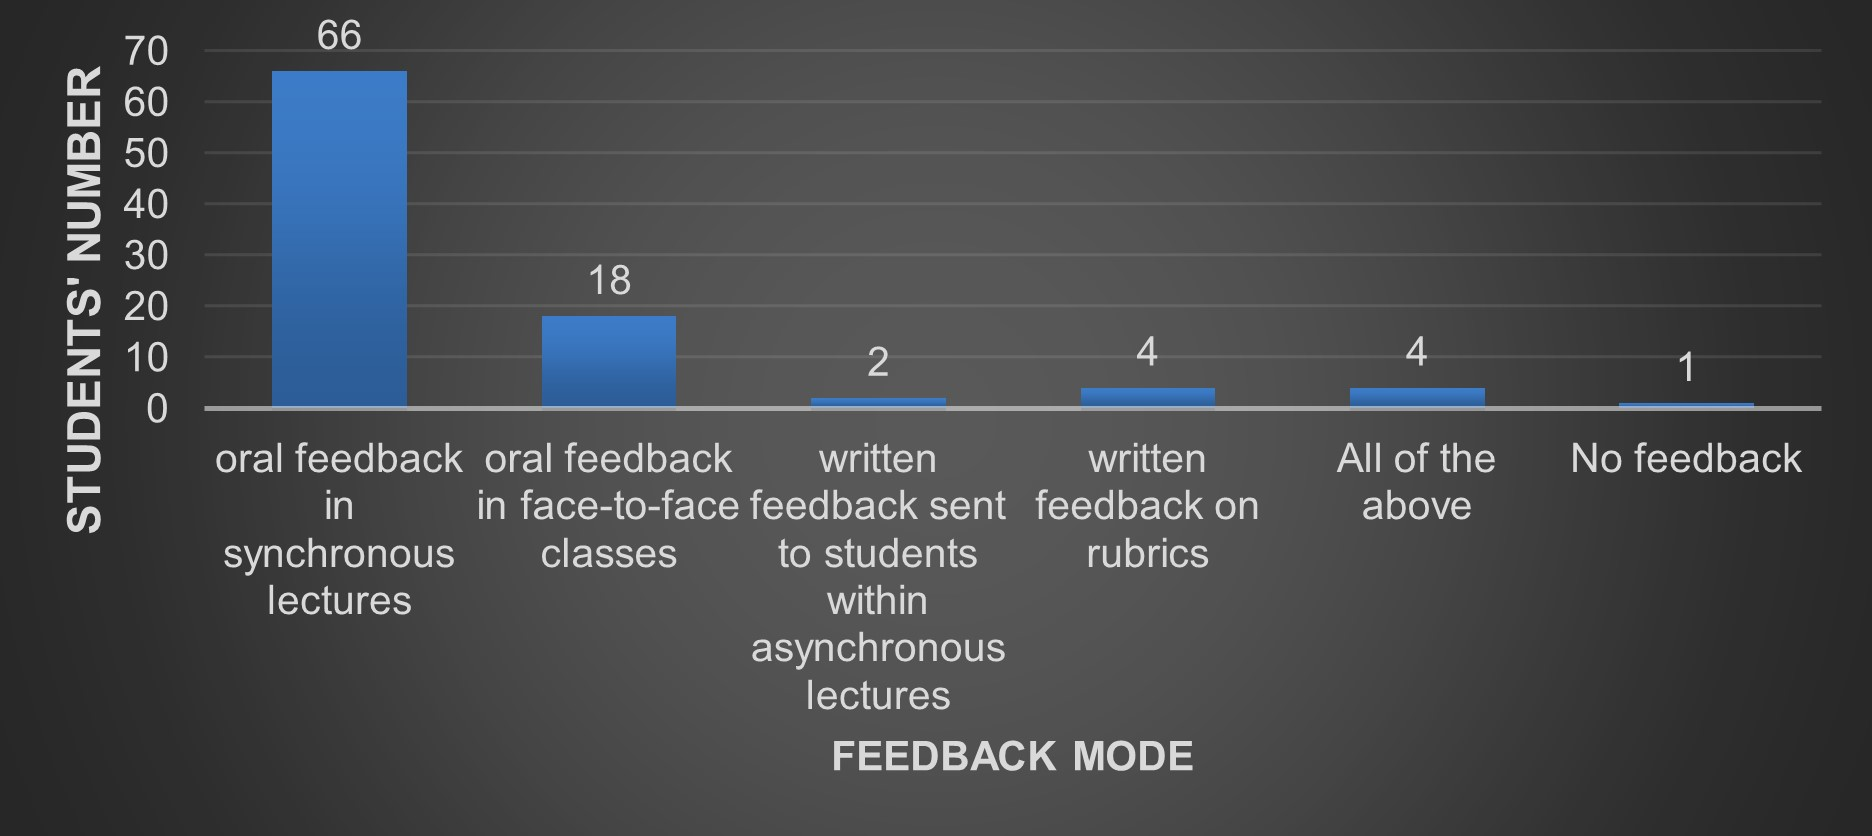
\includegraphics[width=\textwidth]{01.jpg}
 \caption{Feedback mode.}
 \label{fig01}
 \source{Own elaboration.}
 \end{minipage}
\end{figure}


Regarding the aspects covered by teacher feedback, “meaning” was the main category, followed by grammar and paralinguistic skills. This is logical because delivering the message to the audience is the main purpose of the interpreter. Paralinguistic skills related to non-verbal communication, such as maintaining eye contact with the audience and/or speakers, facial expressions, body movement, posture, and voice\footnote{Jeanne Segal, Ph.D., Melinda Smith, M. A., Lawrence Robinson, and Greg Boose, Nonverbal Communication and Body Language, (October 2020). HelpGuide.Org. Available on: \url{https://www.helpguide.org/articles/relationships-communication/nonverbal-communication.htm\#}. Accessed on: 20 Sept. 2021.} were explained to students by providing examples via virtual and conventional classes. However, Krapivkina’s empirical study showed that public speaking is the most challenging area for student interpreters \cite[p. 695]{krapivkina_sight_2018} (\Cref{tbl2}, \Cref{fig02}).

\begin{table}[h!]
\centering
\begin{threeparttable}
\caption{Aspects covered by feedback.}
\label{tbl2}
\centering
\begin{tabular}{p{0.4\textwidth} c c}
\toprule
 & Number of students & Percentage \% \\ \midrule
grammar & 26 & 29.47  \\ 
meaning (accuracy, choice of vocabulary) & 40 & 42.10 \\
paralinguistic features (fluency, pronunciation, intonation. etc.) & 27 & 28.42 \\
Total & 95 & 100 \\
\bottomrule
\end{tabular}
\source{Own elaboration.}
\end{threeparttable}
\end{table}

\begin{figure}[h!]
 \centering
 \begin{minipage}{.85\textwidth}
 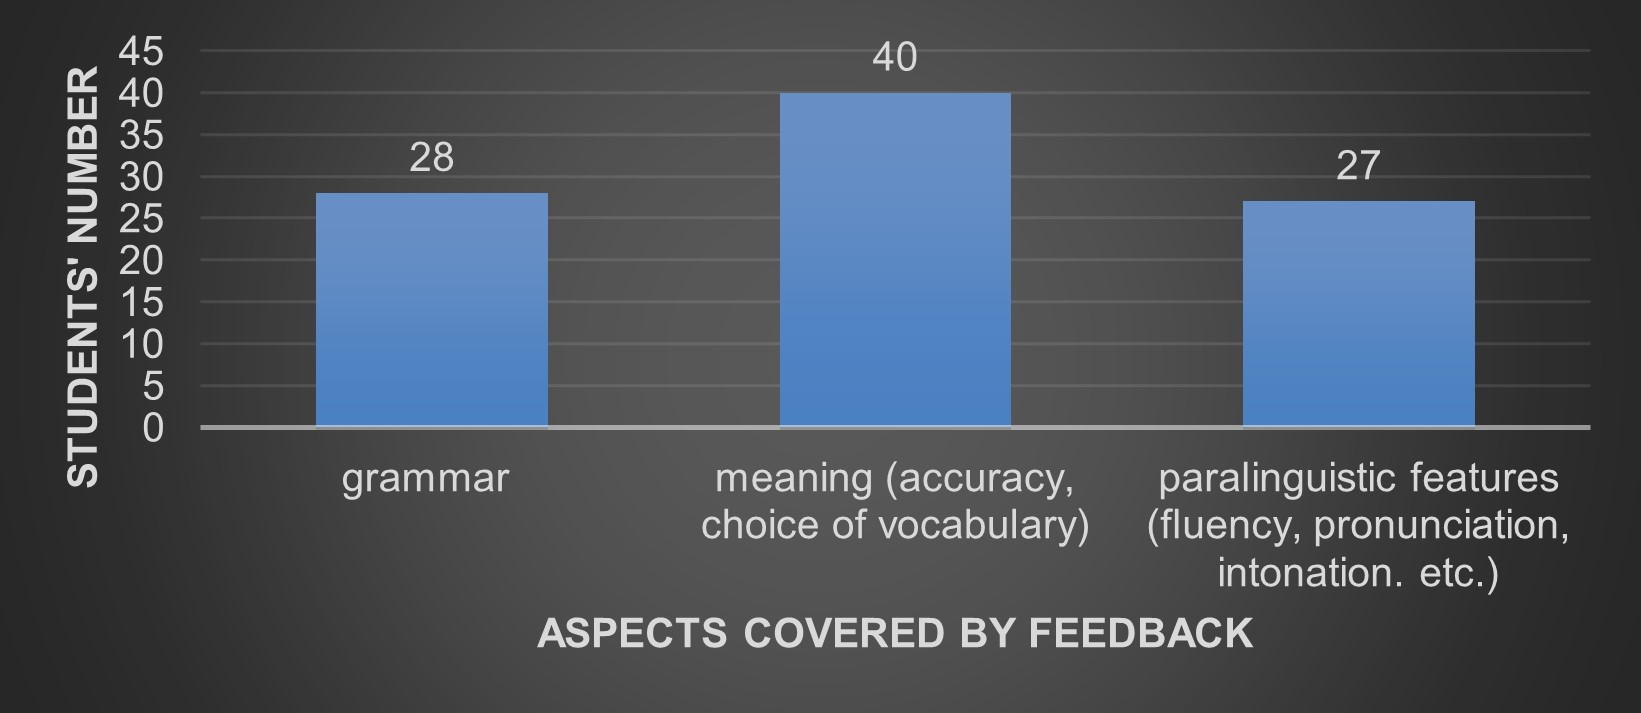
\includegraphics[width=\textwidth]{02.jpg}
 \caption{Aspects covered by feedback.}
 \label{fig02}
 \source{Own elaboration.}
 \end{minipage}
\end{figure}

According to students’ responses, this teacher feedback includes both praise and criticism. Seventeen students answered that they received only praise on their performance, probably because they usually produce good interpretations. Only seven stated that they received criticism probably because they did not perform well at the level of meaning, structure, or paralinguistic features. However, instructors should find a way to make their comments sound more favorable to low achievers (\Cref{tbl3}, \Cref{fig03}).

\begin{table}[h!]
\centering
\begin{threeparttable}
\caption{Praise and criticism in feedback.}
\label{tbl3}
\centering
\begin{tabular}{p{0.2\textwidth} c c}
\toprule
 & Number of students & Percentage \% \\ \midrule
Praise & 17 & 17.89  \\ 
Criticism & 7 & 7.36 \\
Both & 71 & 74.73 \\
Total & 95 & 100 \\
\bottomrule
\end{tabular}
\source{Own elaboration.}
\end{threeparttable}
\end{table}

\begin{figure}[h!]
 \centering
 \begin{minipage}{.85\textwidth}
 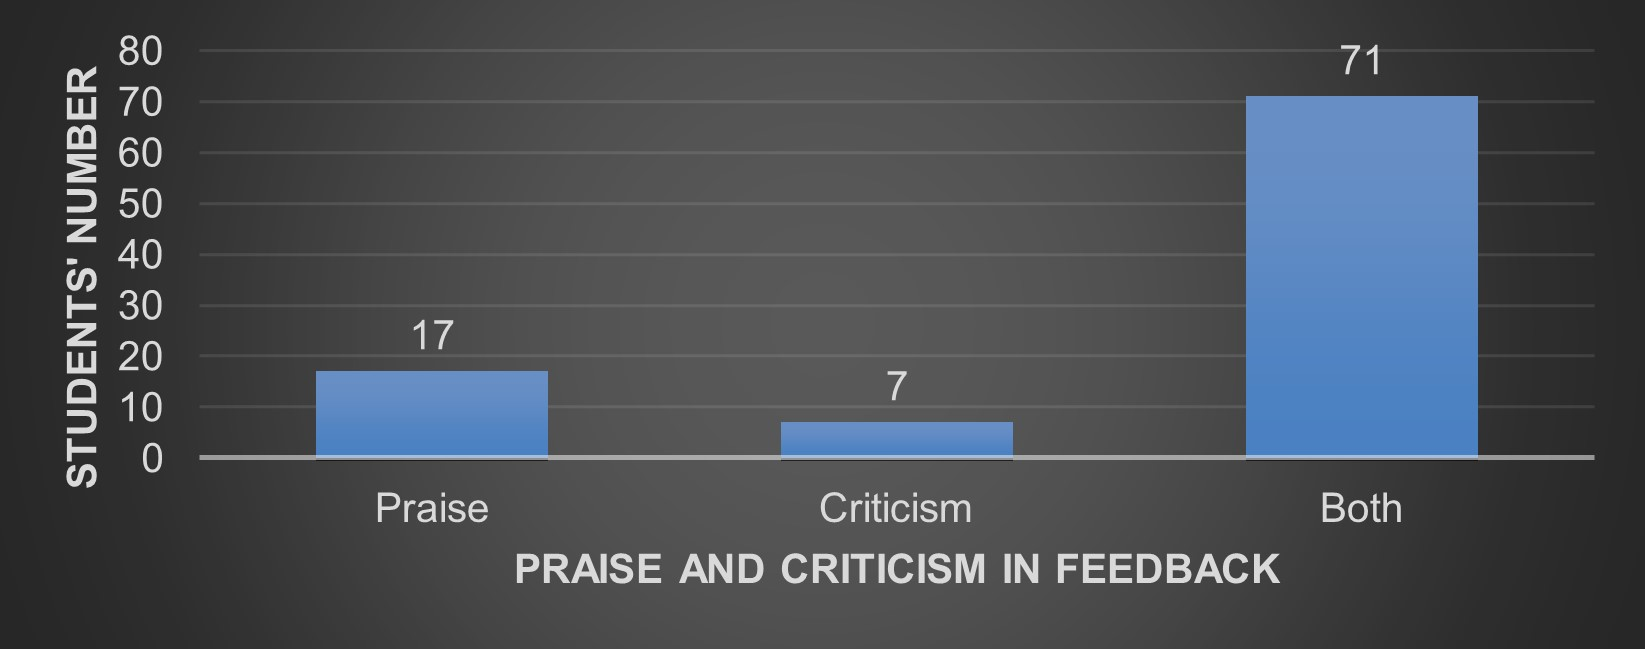
\includegraphics[width=0.85\textwidth]{03.jpg}
 \caption{Praise and Criticism in feedback.}
 \label{fig03}
 \source{Own elaboration.}
 \end{minipage}
\end{figure}

\subsection{Effectiveness of feedback at the cognitive level}

\subsubsection{Understanding the feedback}
Most students stated they were able to fully understand teacher comments online. Few (14) said they could understand but not properly. A very small number (3) reported that teacher feedback was not understandable. The \Cref{tbl4} and \Cref{fig04} show the results:

\begin{table}[h!]
\centering
\begin{threeparttable}
\caption{Feedback is understandable.}
\label{tbl4}
\centering
\begin{tabular}{p{0.2\textwidth} c c}
\toprule
 & Number of students & Percentage \% \\ \midrule
I agree & 78 & 82.10 \\
I partially agree & 14 & 14.73 \\
I do not agree & 3 & 3.15 \\
Total & 95 & 100 \\
\bottomrule
\end{tabular}
\source{Own elaboration.}
\end{threeparttable}
\end{table}

\begin{figure}[h!]
 \centering
 \begin{minipage}{.85\textwidth}
 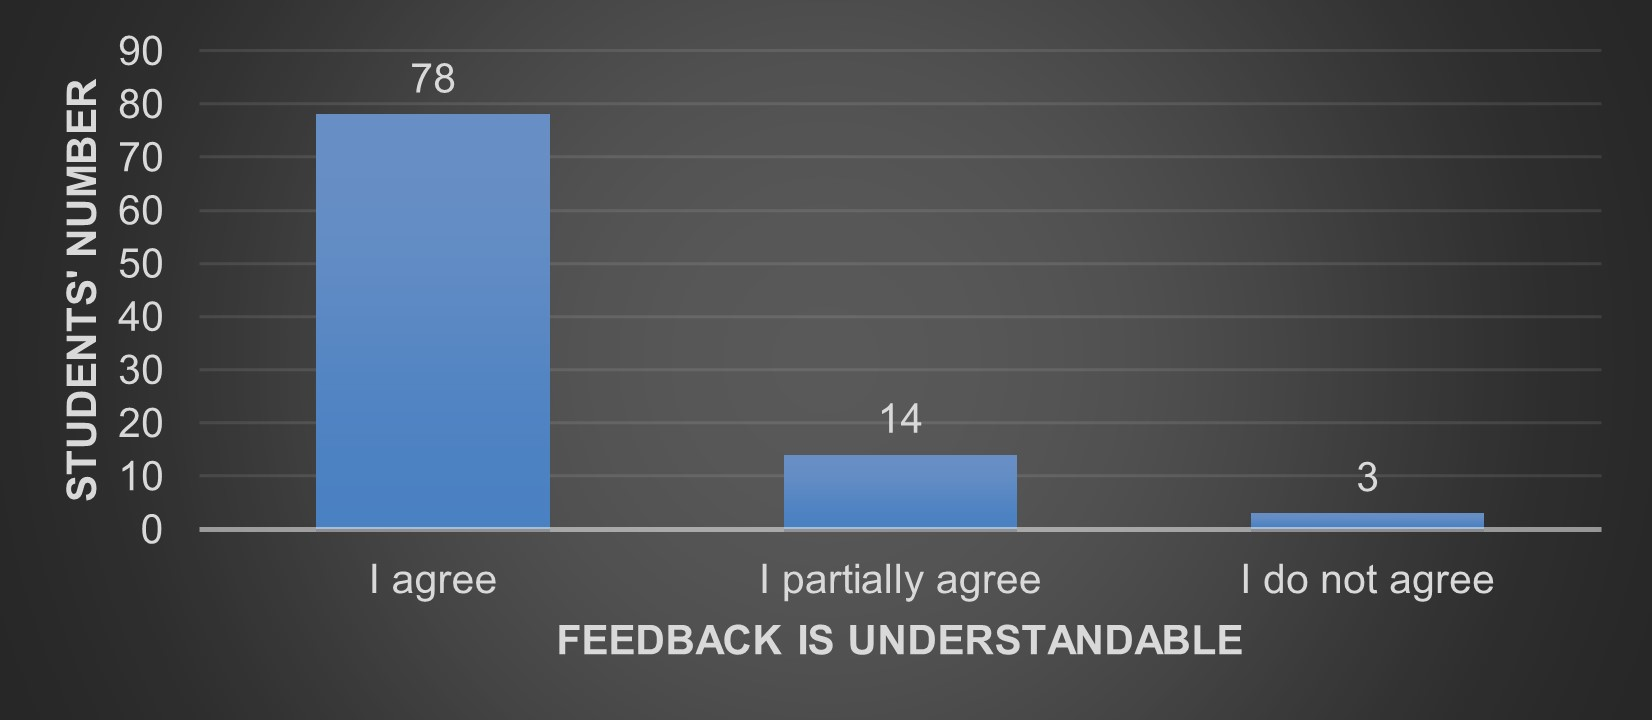
\includegraphics[width=\textwidth]{04.jpg}
 \caption{Feedback is understandable.}
 \label{fig04}
 \source{Own elaboration.}
 \end{minipage}
\end{figure}

Compared to face-to-face feedback, most students reported that it is equally understandable or even more understandable (\Cref{tbl5} and \Cref{fig05}). This reveals that the virtual mode did not affect them. Moreover, some of them focused better online, either because they are auditory learners who feel very comfortable with audio resources for learning or because in virtual classrooms, unlike conventional ones, side talk between students is not possible, which \textcite[p. 828]{ko_teaching_2009} considers as an advantage. However, 21 students expressed that online feedback is less understandable probably for cognitive, technical, or environmental reasons. They might be visual learners, who need visual interaction, they experienced technical issues, like poor sound quality, inability to use digital tools effectively, or the noise in their environment, usually the family home, distracted them. (See \textcite{naqeeb_learning_2011}, on auditory, visual and other learning styles).

\begin{table}[h!]
\centering
\begin{threeparttable}
\caption{Comparison with face-to-face feedback.}
\label{tbl5}
\centering
\begin{tabular}{p{0.3\textwidth} c c}
\toprule
 & Number of students & Percentage \% \\ \midrule
Equally understandable & 50 & 52.63 \\
Less understandable & 21 & 22.10 \\
More understandable & 24 & 25.26 \\
Total & 95 & 100 \\
\bottomrule
\end{tabular}
\source{Own elaboration.}
\end{threeparttable}
\end{table}

\begin{figure}[h!]
 \centering
 \begin{minipage}{.85\textwidth}
 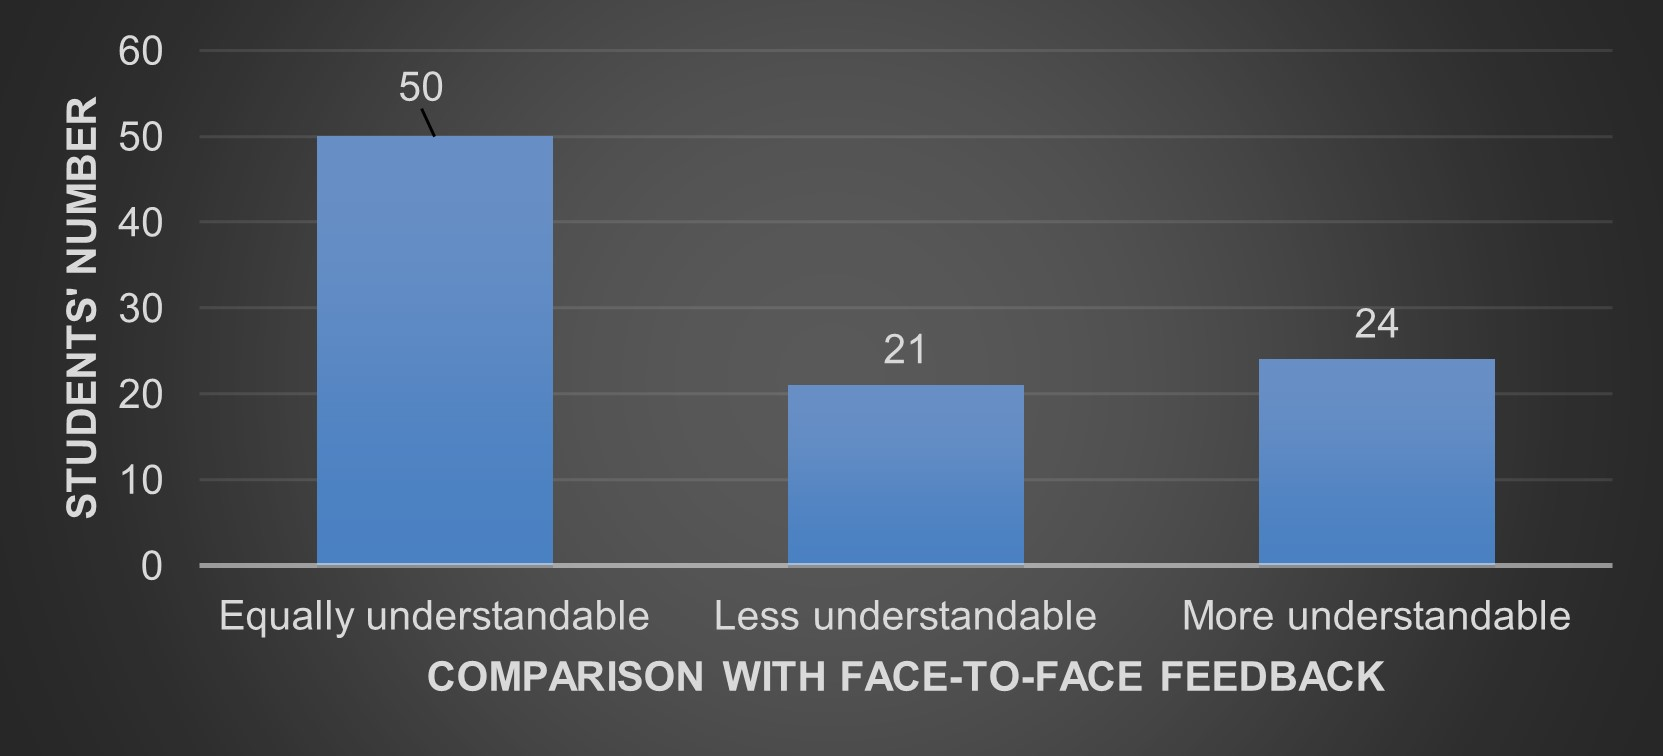
\includegraphics[width=\textwidth]{05.jpg}
 \caption{Comparison with face-to-face feedback.}
 \label{fig05}
 \source{Own elaboration.}
 \end{minipage}
\end{figure}

\textcite[p. 826]{ko_teaching_2009} explains that “background noise” from the “surrounding environment” may come from different sources, like persons, TV, or household work, and students may need time to overcome this problem. Another influential factor that decreases concentration and capacity to receive and understand feedback is fatigue in remote interpreting settings. It also affects professional interpreters. According to \textcite[p. 9]{karaban_exploring_2021}, they face various challenges in addition to fatigue due to the “unfamiliar interpreting settings”, especially during the pandemic, when many interpreting services are provided remotely. The researchers state that specific training can help to overcome “mental and cognitive issues” that may arise.  Some researchers have mentioned problems related to “poor concentration”, “stress” and fatigue in the absence of “visual interaction” \cite[p. 827]{ko_teaching_2009}. Indeed, one student reported diminished concentration abilities and attention span in the distance learning mode. However, during his experiment of “teaching interpreting by distance mode”, \textcite[p. 827]{ko_teaching_2009} observed that online students encountered the problem of “a shorter attention span” at the beginning, but gradually became familiar with the settings and the devices used. He suggested a period of six weeks or 18 hours and more to increase the training’s effectiveness and improve the “concentration span”. In our case, the training program lasted more than six weeks, and our findings were consistent with \posscite{ko_teaching_2009} study, although a small number of students did not get used to this new environment. Other external factors, such as “the close ties between family members” and “positive environmental support” help students address the difficulties of online learning \cite[p. 16]{susilana_studentsa_2020}.


\subsubsection{Using the feedback}
Scholars agree that effective feedback does not involve only the teacher giving comments to the learners but also students understanding and using those comments \cite{carless_development_2018,ryan_feedback_2019}. Feedback usability is considered one of the “valuable indicators of feedback success” \cite[p. 1519]{ryan_feedback_2019}. Therefore, the learner should be able to interpret timely, detailed, and specific feedback comments. For example, instructors use recorded audios to highlight strengths and weaknesses with real examples from students’ works \cite{henderson_conditions_2019}. In this regard, \textcite[p. 1509]{ryan_feedback_2019} argued that “the combination of detail, personalization, and usability are synergistic”. While detail and personalization are not enough to lead to feedback usability, they can affect its benefit for subsequent work. To this end, teachers may rely on different means, like digitally recorded or written feedback sent outside classes.  Our findings indicated that few students managed to identify their errors and understand their nature, whereas a greater number also reflected on them, by understanding their causes, and finding ways to remedy them. According to \textcite[p. 1322]{carless_development_2018}, information is considered feedback “only when students act on it”. In our case, most students could make sense of the feedback and use it in future tasks. This stresses their active role in the feedback process (\Cref{tbl6}, \Cref{fig06}).

\begin{table}[h!]
\centering
\begin{threeparttable}
\caption{Feedback enables students to.}
\label{tbl6}
\centering
\begin{tabular}{p{0.4\textwidth} c c}
\toprule
 & Number of students & Percentage \% \\ \midrule
identify error(s) only & 13 & 13.68 \\
reflect on errors & 23 & 24.21 \\
use the comments in  future tasks & 59 & 62.10 \\
Total & 95 & 100 \\
\bottomrule
\end{tabular}
\source{Own elaboration.}
\end{threeparttable}
\end{table}

\begin{figure}[h!]
 \centering
 \begin{minipage}{.85\textwidth}
 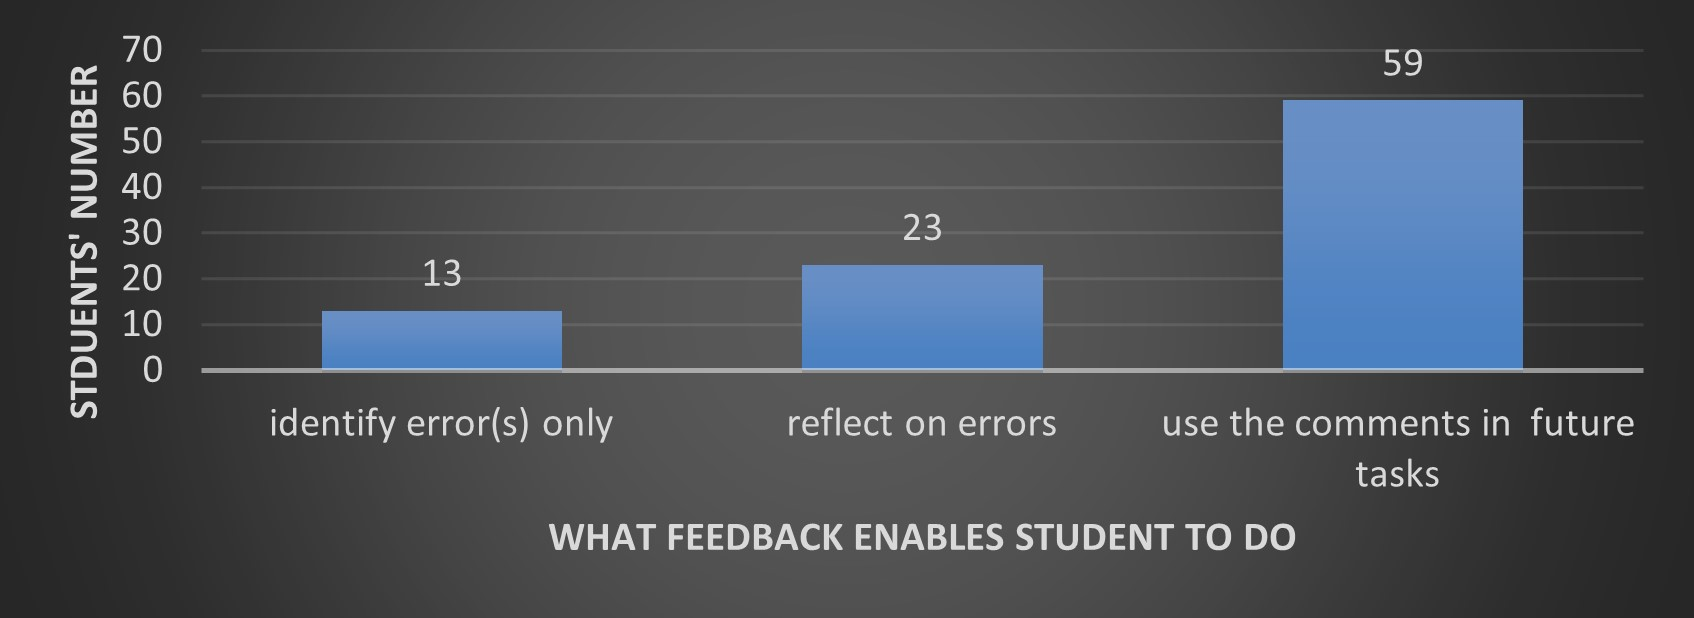
\includegraphics[width=\textwidth]{06.jpg}
 \caption{What feedback enables students to do.}
 \label{fig06}
 \source{Own elaboration.}
 \end{minipage}
\end{figure}


\Cref{tbl7} and \Cref{fig07} also indicate that not all students can act on the feedback received. According to \textcite[p. 1318]{carless_development_2018}, “students need to possess a repertoire of strategies to act productively”. Furthermore, most students (77) believed that feedback helps improve performance, especially at the level of structure, then accuracy, and finally paralinguistic features (\Cref{tbl8}, \Cref{fig08}).

\begin{table}[h!]
\centering
\begin{threeparttable}
\caption{Feedback improves performance.}
\label{tbl7}
\centering
\begin{tabular}{p{0.5\textwidth} c c}
\toprule
Feedback is beneficial and helps you improve your performance & Number of students & Percentage \% \\ \midrule
I agree & 77 & 81.05 \\
I partially agree & 15 & 15.78 \\
I do not agree & 3 & 3.15 \\
Total & 93 & 100 \\
\bottomrule
\end{tabular}
\source{Own elaboration.}
\end{threeparttable}
\end{table}

\begin{figure}[h!]
 \centering
 \begin{minipage}{.85\textwidth}
 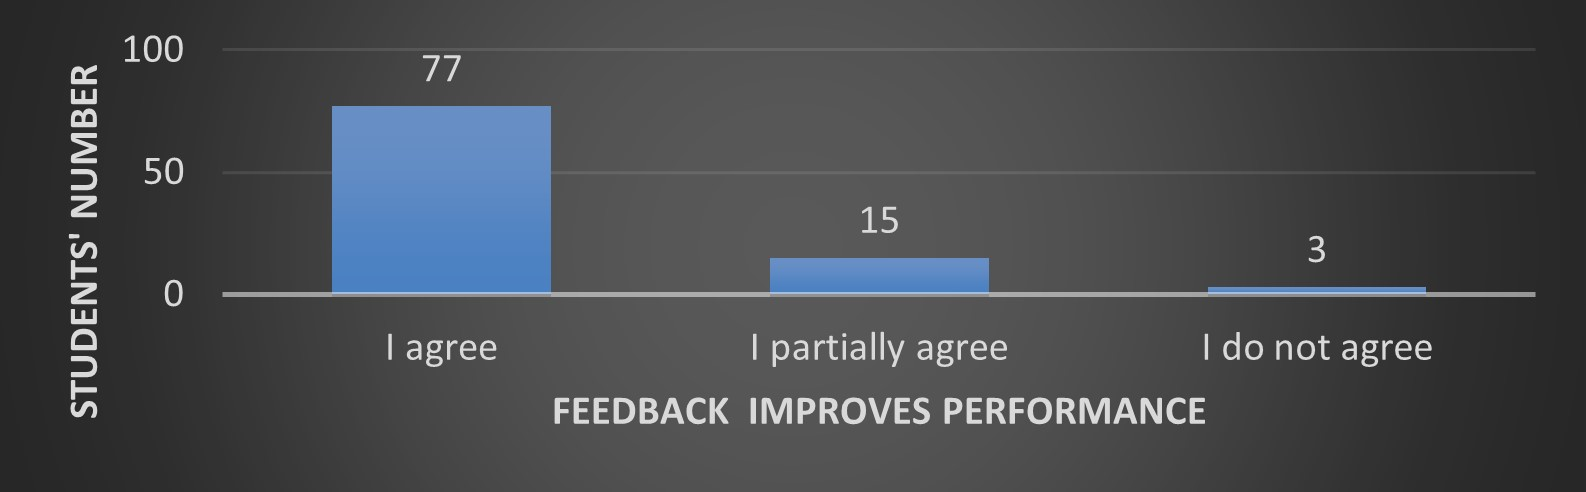
\includegraphics[width=\textwidth]{07.jpg}
 \caption{Feedback improves performance.}
 \label{fig07}
 \source{Own elaboration.}
 \end{minipage}
\end{figure}

\begin{table}[h!]
\centering
\begin{threeparttable}
\caption{What it improves.}
\label{tbl8}
\centering
\begin{tabular}{p{0.4\textwidth} c c}
\toprule
What it improves & Number of students & Percentage \% \\ \midrule
production becomes more accurate & 32 & 34.40 \\
You build constructions more correctly & 43 & 46.23 \\
paralinguistic skills improve & 18 & 19.35 \\
Total & 95 & 100 \\
\bottomrule
\end{tabular}
\source{Own elaboration.}
\end{threeparttable}
\end{table}

\begin{figure}[h!]
 \centering
 \begin{minipage}{.85\textwidth}
 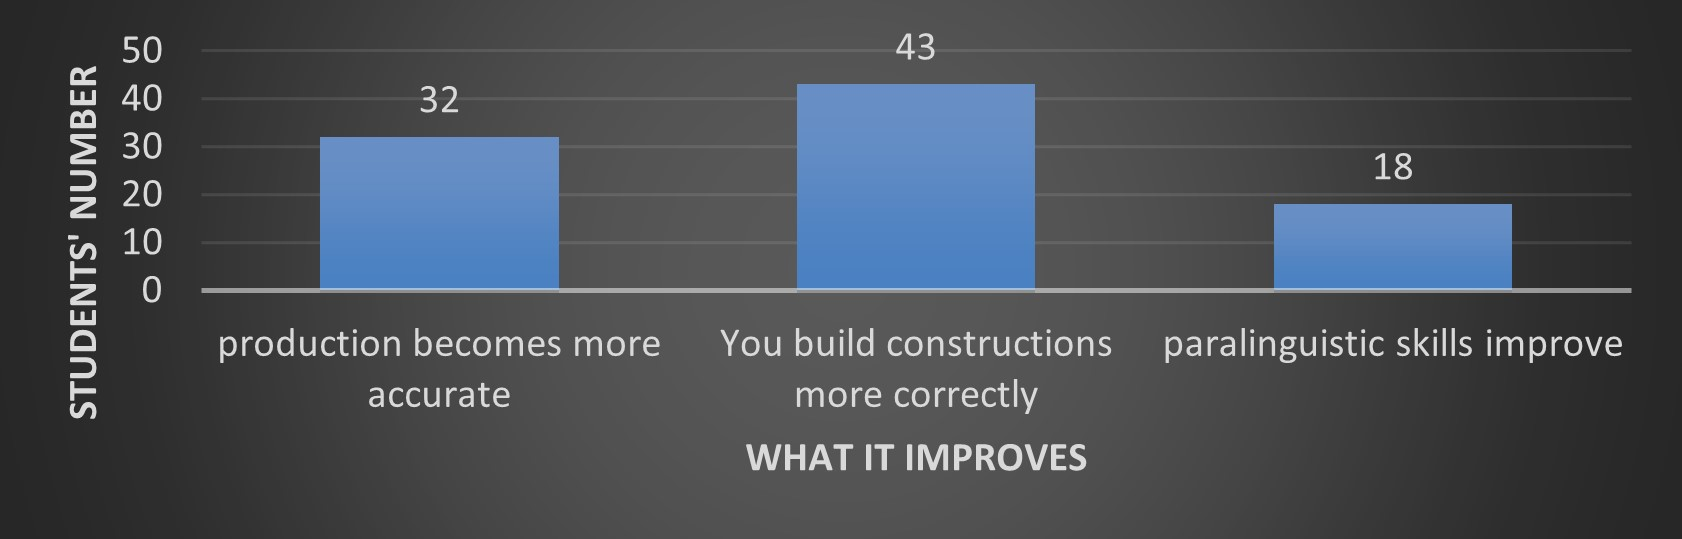
\includegraphics[width=\textwidth]{08.jpg}
 \caption{What it improves.}
 \label{fig08}
 \source{Own elaboration.}
 \end{minipage}
\end{figure}

This can be explained by the fact that the most significant number of errors are made in the structure, particularly in the Arabic to English interpretation. This does not necessarily reflect a gap in knowledge but a problem with internalizing specific structures from the second language (On internalization see \cite{chappell_sociocultural_2012}). Concerning paralinguistic issues, like “demonstrating inappropriate body language and maintaining an inappropriate level of eye contact” \cite[p. 821]{ko_teaching_2009}, we believe that it is more difficult for the teacher to provide feedback in this area, especially when only audio is used. As for the time interval needed by students to apply the comments in subsequent learning activities and assignments, 52.68 \% responded that a short period (1 week- 1 month) is sufficient (\Cref{tbl9}, \Cref{fig09}):

\begin{quote}
     There was a lot more fluency in my final exam translation. I liked how better I got in a short amount of time.
\end{quote}

\begin{table}[h!]
\centering
\begin{threeparttable}
\caption{Time period needed to use feedback.}
\label{tbl9}
\centering
\begin{tabular}{p{0.5\textwidth} c c}
\toprule
 & Number of students & Percentage \% \\ \midrule
On a short–term period (1 week-1 month) & 49 & 52.68 \\
On a long-term period (1 month or more) & 44 & 47.31 \\
Total & 93 & 100 \\
\bottomrule
\end{tabular}
\source{Own elaboration.}
\end{threeparttable}
\end{table}

\begin{figure}[h!]
 \centering
 \begin{minipage}{.6\textwidth}
 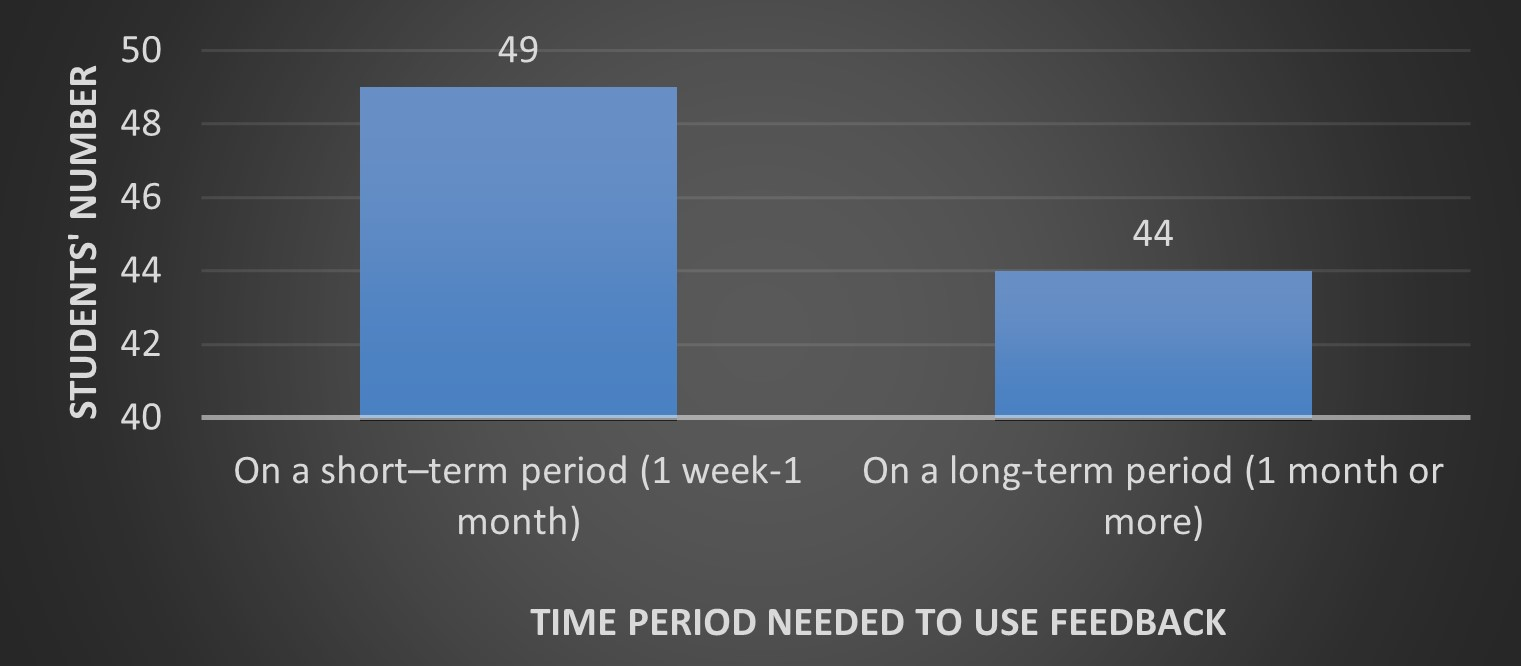
\includegraphics[width=\textwidth]{09.jpg}
 \caption{Time period needed to use feedback.}
 \label{fig09}
 \source{Own elaboration.}
 \end{minipage}
\end{figure}

Their answers to the question that comes after indicated that they remember the teacher’s comments and use them immediately during individual practice outside the classes or in subsequent lectures. They try to avoid mistakes or self-correction in areas including fluency, pronunciation, tone, the choice of words, accuracy, structure and word order, global performance, and confidence in delivery. Comments were also helpful to them during exams. Meanwhile, 47.31 \% answered that a more extended period is needed. They used the comments in later stages, such as in the “consecutive interpreting” during the following semester. This demonstrates the long-term positive effect of feedback.

\subsection{Effectiveness of feedback at the emotional level}

\subsubsection{Interaction}
Forty-six students maintained that the interaction prompted by online feedback is similar to that in on-campus classes:

\begin{quote}
All we need are verbal comments which are provided in online feedback as well as face-to-face feedback, so there’s no difference.  
\end{quote}

Students state that they can still discuss several aspects of the interpretations produced with their teachers, and the communication process remains the same, although 29 students believe communication became less effective because visual interaction is essential for good communication; they think face-to-face contact offers more diversity and enables students to exchange views with each other; therefore, it is more effective:

\begin{quote}
    In on-campus classes, the sound is clearer, and I can see people's reactions.
    
Online classes limit our productivity. Some students may not pay attention because they do not feel that their homes provide the same environment as the university.

Peer interaction is lower.

I experience more anxiety when I try to participate online.
\end{quote}

What is surprising is that 18 students thought online interaction was higher. They feel more comfortable with the virtual settings and consider them more interactive, making discussion richer and more intense. They listen more attentively and may become more motivated and encouraged to participate. According to them, face-to-face contact triggers feelings of shyness, insecurity, and reduces self-confidence:

\begin{quote}
    It's easier to discuss when you're not in front of the students.
\end{quote}

Some students feel stressed and embarrassed when talking in front of the teacher and peers, but things become easier in the distance mode, and the student gains more confidence.

\begin{quote}
    I couldn’t interact with the teacher and my classes and could not develop my skills due to fear and anxiety. But thanks to online lectures, I gained self-confidence and managed to participate and process feedback.
\end{quote}

One student answered that interaction outside the class is also important by contacting the teacher via email, WhatsApp, and Microsoft Teams and it is better than visiting the teacher during office hours (\Cref{tbl10}, \Cref{fig10}).

\begin{table}[h!]
\centering
\begin{threeparttable}
\caption{Comparison of interaction levels prompted by online and face-to-face feedback modes.}
\label{tbl10}
\begin{tabular}{p{0.1\textwidth} c c}
\toprule
 & Number of students & Percentage \% \\ \midrule
Equal & 46 & 49.46 \\
lower & 29 & 31.18 \\
Higher & 18 & 19.35 \\
Total & 93 & 100 \\
\bottomrule
\end{tabular}
\source{Own elaboration.}
\end{threeparttable}
\end{table}

\begin{figure}[h!]
 \centering
 \begin{minipage}{.85\textwidth}
 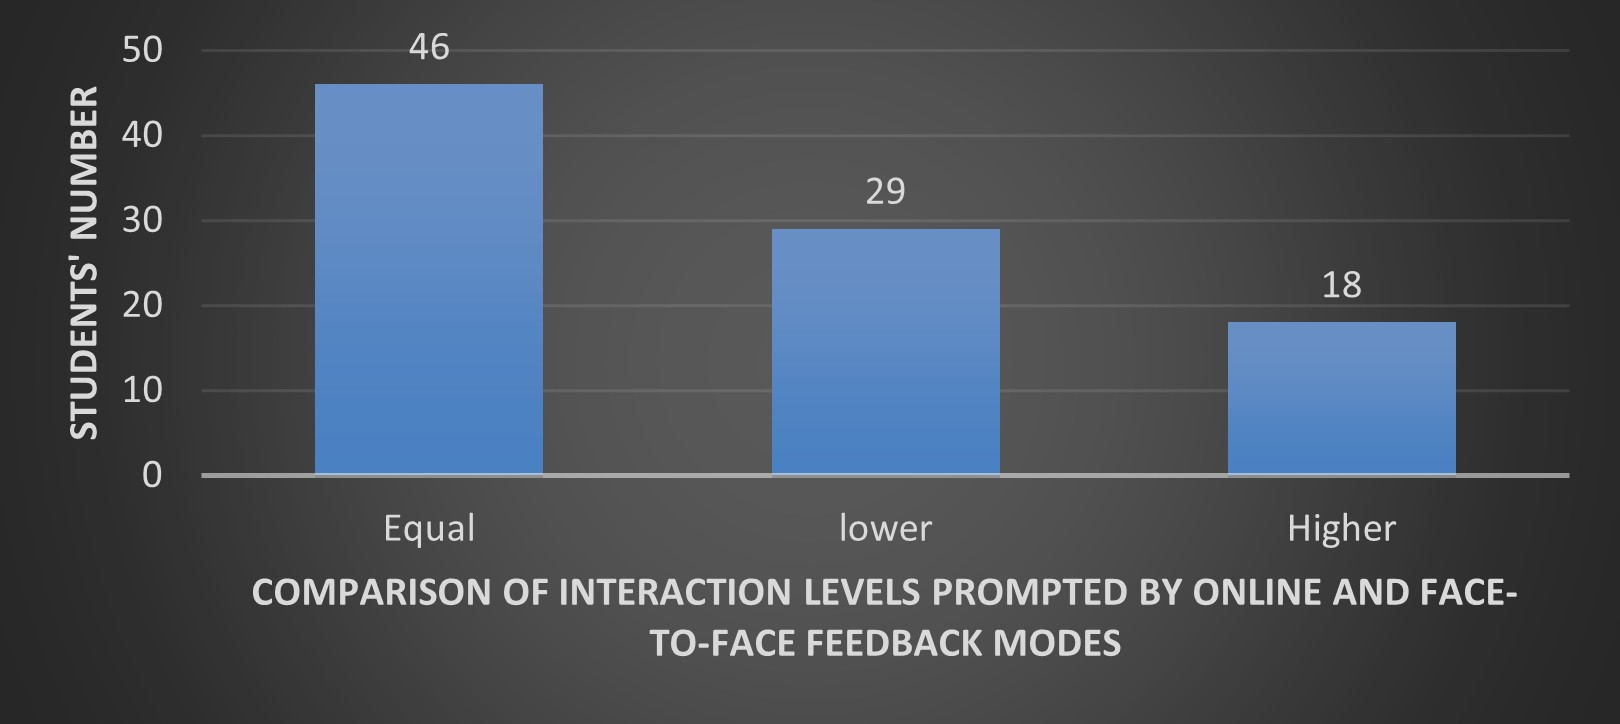
\includegraphics[width=\textwidth]{10.jpg}
 \caption{Comparison of interaction levels prompted by online and face-to-face feedback modes.}
 \label{fig10}
 \source{Own elaboration.}
 \end{minipage}
\end{figure}

\subsubsection{Engagement}
Engagement is “the degree of attention, curiosity, interest, optimism, and passion that students show when they are learning or being taught”1. Feedback may have a positive influence on engagement \cite[p. 30]{ogange_student_2018}. Fifty-two students believed online feedback stimulates an engagement similar to that received in a traditional classroom. They noted that comments are the same; therefore, they can assimilate them and use them regardless of the mode. Furthermore, they pointed out that interpreting is an oral activity that requires the auditory input only:

\begin{quote}
    My reaction is the same in both modes.
    
I want to have good grades, so my engagement is the same.
\end{quote}

On the other hand, 15 students thought that engagement is lower in the off-campus mode. The distance mode is more challenging and makes studying more exhausting. The absence of visual interaction affects learning negatively, and technical issues, poor connection, and the distractions associated with the online mode may lead to poor concentration:

\begin{quote}
    It requires more personal effort from the student to become industrious and engaged.
\end{quote}

Twenty-five students believed their engagement is higher in virtual settings:

\begin{quote}
    The teacher’s voice is clear and heard by everyone.
    
Getting ready for the lectures has improved with online learning.

With online lectures, I concentrate better and make more progress.
\end{quote}

One student stressed the importance of feedback specificity and believed that it contributes to her engagement. Another one highlighted the “clarity” of the teacher’s message as an essential factor regardless of the mode (\Cref{tbl11}, \Cref{fig11}).

\begin{quote}
    If the feedback is given to me specifically, then I take it into consideration.
\end{quote}

\begin{table}[h!]
\centering
\begin{threeparttable}
\caption{Engagement with online feedback compared to face-to-face feedback.}
\label{tbl11}
\begin{tabular}{p{0.1\textwidth} c c}
\toprule
 & Number of students & Percentage \% \\ \midrule
Equal & 52 & 56.52 \\
Lower & 15 & 16.30 \\
Higher & 25 & 27.17 \\
Total & 92 & 100 \\
\bottomrule
\end{tabular}
\source{Own elaboration.}
\end{threeparttable}
\end{table}

\begin{figure}[h!]
 \centering
 \begin{minipage}{.85\textwidth}
 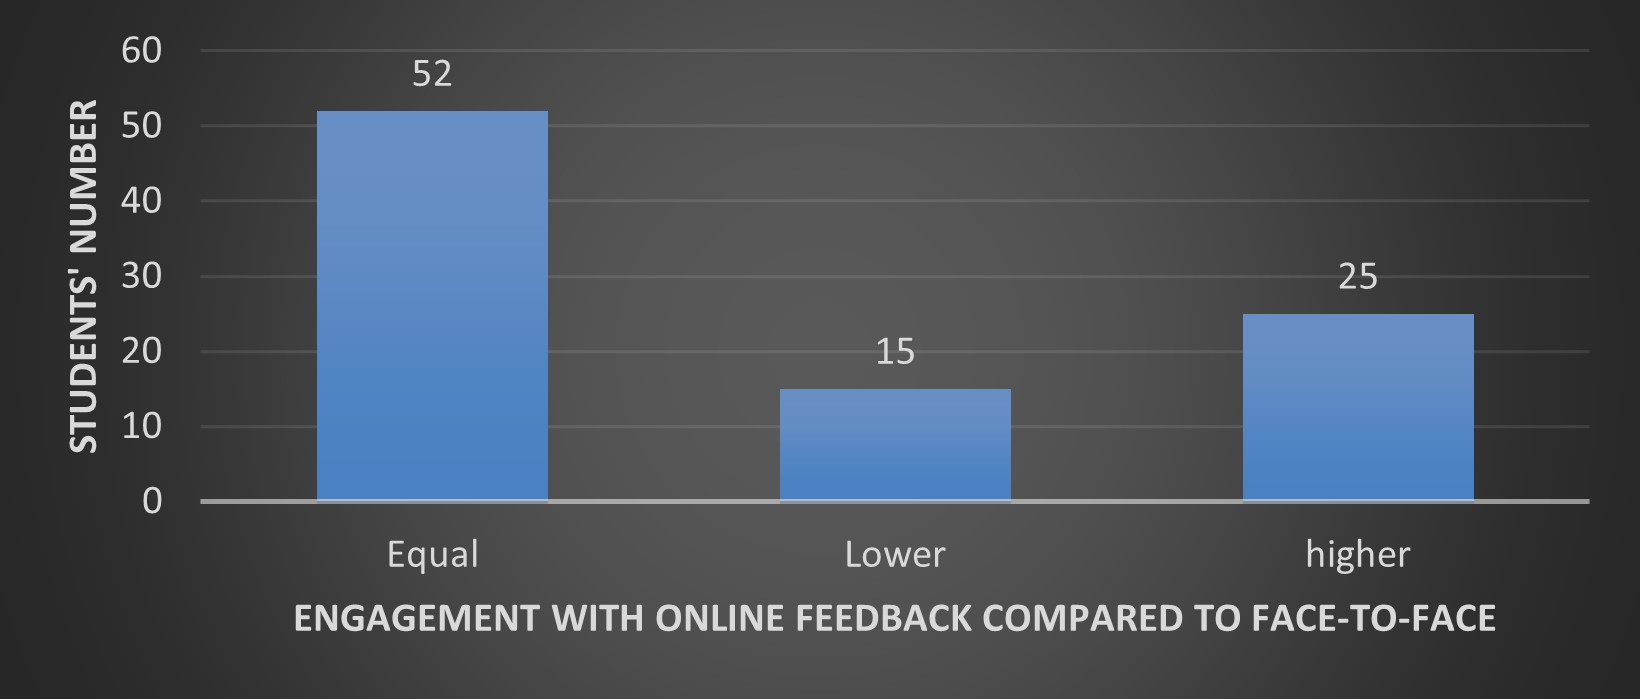
\includegraphics[width=\textwidth]{11.jpg}
 \caption{Engagement with online feedback compared to face-to-face feedback.}
 \label{fig11}
 \source{Own elaboration.}
 \end{minipage}
\end{figure}

\subsubsection{Students’ preferences and expectations}
To understand students’ needs and expectations, we asked them further questions to know which priorities should be addressed when designing efficient educational processes.

Feedback necessity for the teaching and learning process
Ninety students recognized the necessity of feedback in this interpreting course. Only one saw feedback as not necessary, while four did not answer the question (\Cref{tbl12}, \Cref{fig12}).

\begin{table}[h!]
\centering
\begin{threeparttable}
\caption{Feedback is necessary.}
\label{tbl12}
\centering
\begin{tabular}{p{0.1\textwidth} c c}
\toprule
 & Number of students & Percentage \% \\ \midrule
Yes & 90 & 98.90 \\
No & 1 & 1.09 \\
Total & 91 & 100 \\
\bottomrule
\end{tabular}
\source{Own elaboration.}
\end{threeparttable}
\end{table}

\begin{figure}[h!]
 \centering
 \begin{minipage}{.85\textwidth}
 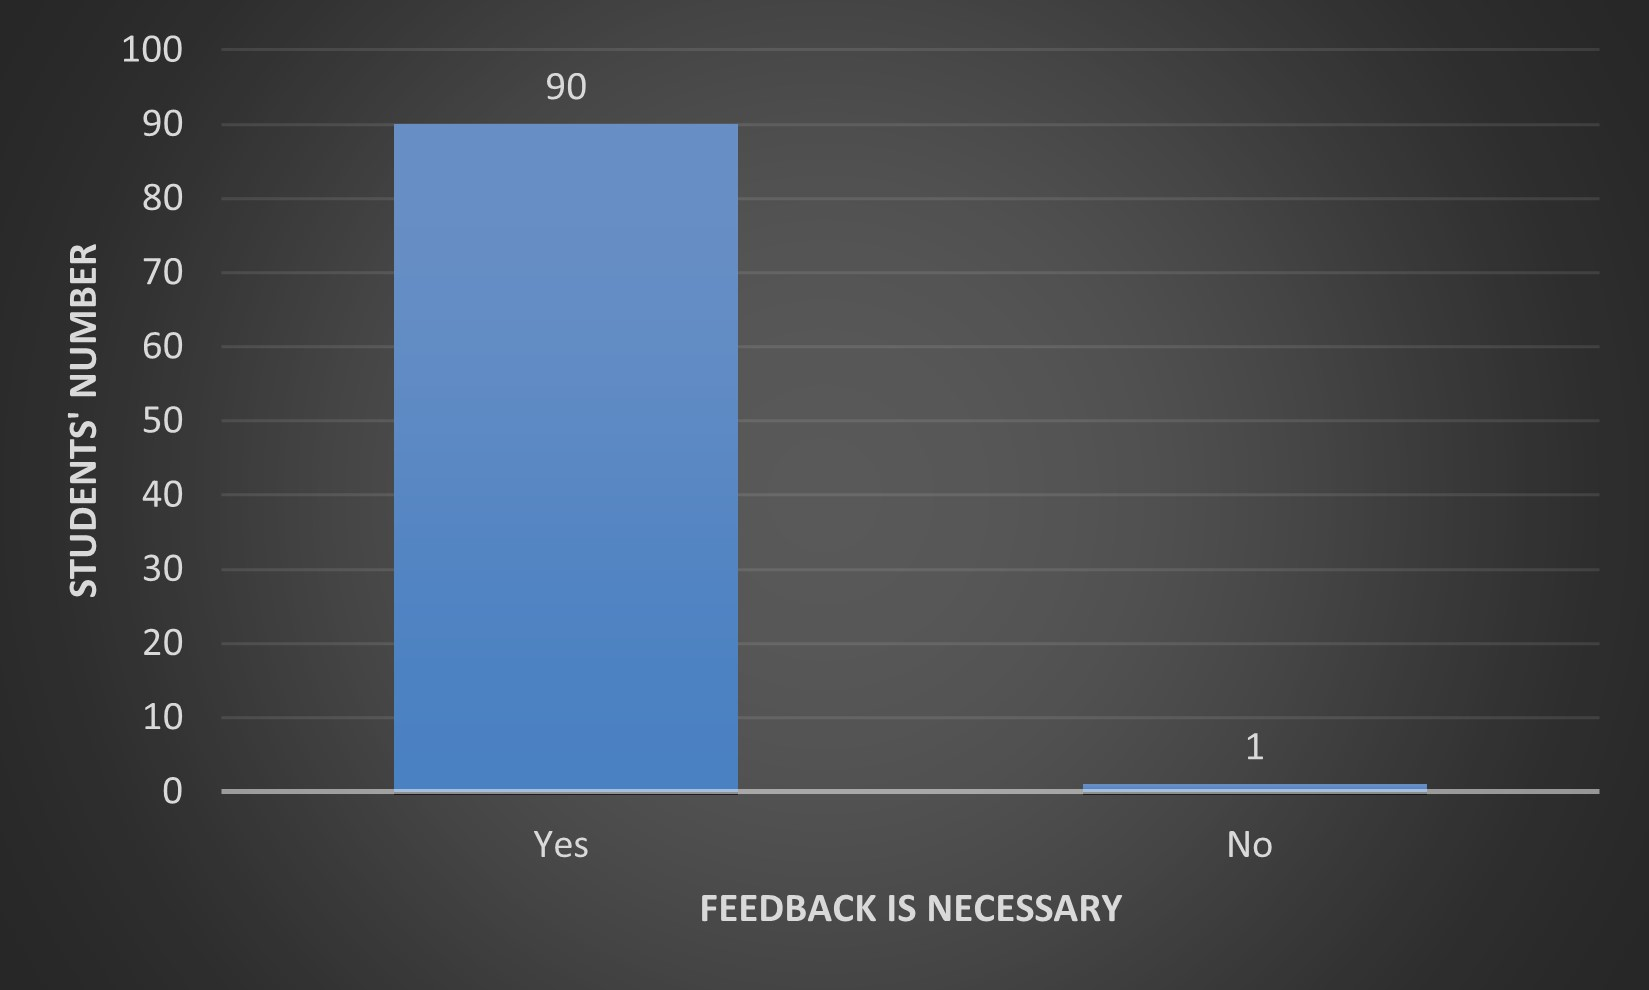
\includegraphics[width=\textwidth]{12.jpg}
 \caption{Feedback is necessary.}
 \label{fig12}
 \source{Own elaboration.}
 \end{minipage}
\end{figure}

We also asked whether teacher feedback has only disadvantages and makes them feel unsafe to uncover their psychological attitudes and needs. \Cref{tbl13} and \Cref{fig13} summarize the results.

\begin{table}[h!]
\centering
\begin{threeparttable}
\caption{Perception of the feedback given in conventional classes.}
\label{tbl13}
\begin{tabular}{p{0.5\textwidth} c c}
\toprule
 & Number of students & Percentage \% \\ \midrule
teacher feedback has only disadvantages and makes you feel in an unsafe
learning environment &  &  \\
I agree & 9 & 9.47 \\
I partially agree & 6 & 6.31 \\
I do not agree & 80 & 84.21 \\
Total & 95 & 100 \\
\bottomrule
\end{tabular}
\source{Own elaboration.}
\end{threeparttable}
\end{table}

\begin{figure}[h!]
 \centering
 \begin{minipage}{.85\textwidth}
 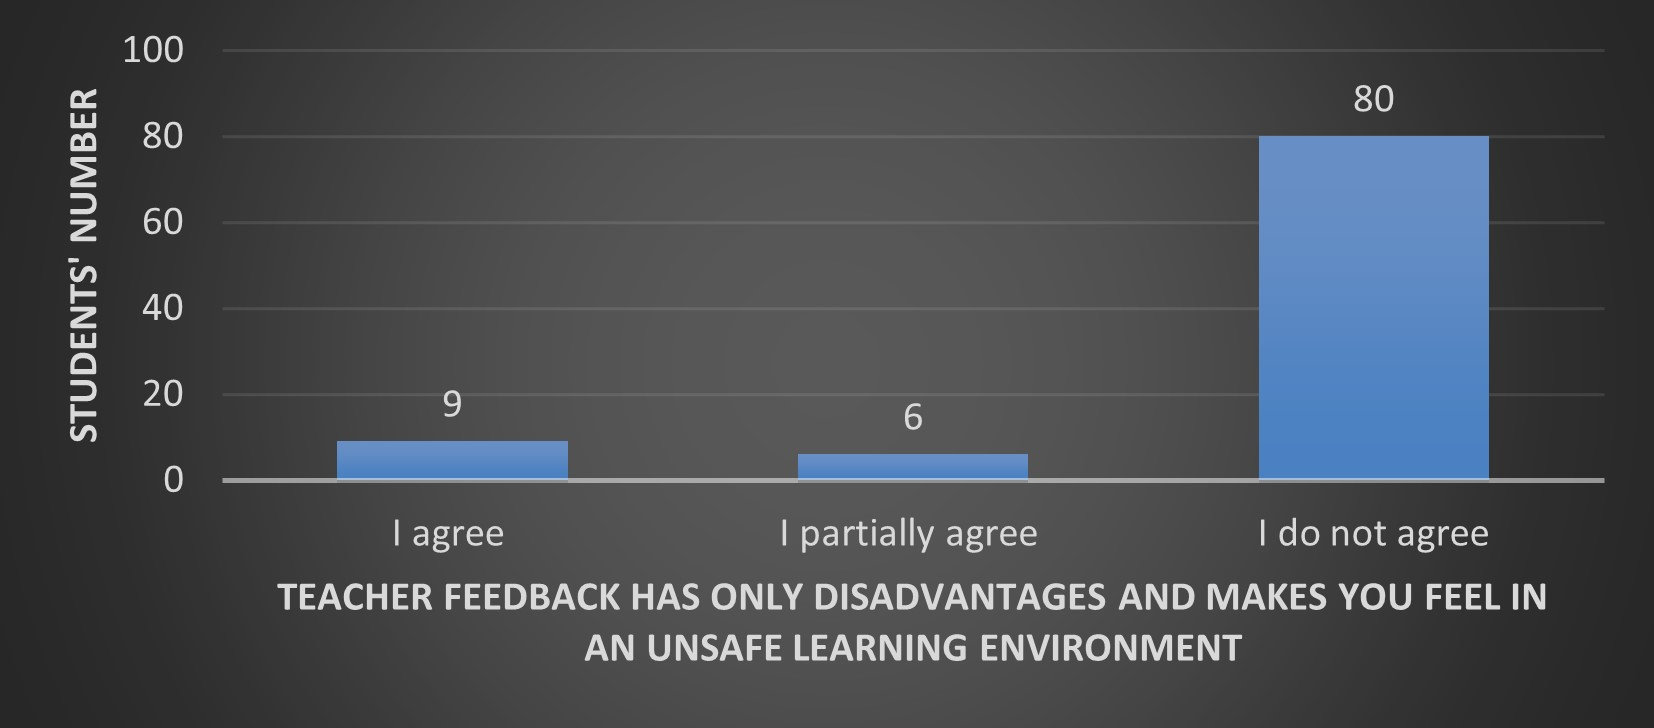
\includegraphics[width=0.85\textwidth]{13.jpg}
 \caption{Perception of the feedback given in conventional classes.}
 \label{fig13}
 \source{Own elaboration.}
 \end{minipage}
\end{figure}

These results suggest that students do not have a problem with feedback itself but probably with the way it is provided. \textcite[p. 796]{leighton_students_2019} explained that “an inherent tension or conflict of interest” between educators and learners may influence both parties in the feedback process. \textcite[p. 1409]{henderson_conditions_2019} also highlighted the “emotional reactions” of both teacher and student in feedback situations pointing out that they might hamper the latter from making sense of feedback. The study of \textcite[p. 163-164]{lee_feedback_2018} revealed that a large number of students need positive and reassuring comments that help them cope with stress and anxiety generated by interpreting training and exams.

Concerning oral feedback in virtual lectures, we asked them whether it enhances learning when provided in front of their classmates, 46 students had a favorable view, eight did not view it as an opportunity, and 37 were undecided. Finally, four students did not answer the question. This indicates that only half of them considered feedback as constructive and beneficial to reinforce learning (\Cref{tbl14}, \Cref{fig14}):

\begin{table}[h!]
\centering
\begin{threeparttable}
\caption{Perception of oral feedback in virtual classes(a).}
\label{tbl14}
\begin{tabular}{p{0.4\textwidth} c c}
\toprule
Feedback is an opportunity for learning & Number of students & Percentage \% \\ \midrule
I agree & 46 & 50.54 \\
I partially agree & 37 & 40.65 \\
I do not agree & 8 & 8.79 \\
Total & 91 & 100 \\
\bottomrule
\end{tabular}
\source{Own elaboration.}
\end{threeparttable}
\end{table}

\begin{figure}[h!]
 \centering
 \begin{minipage}{.85\textwidth}
 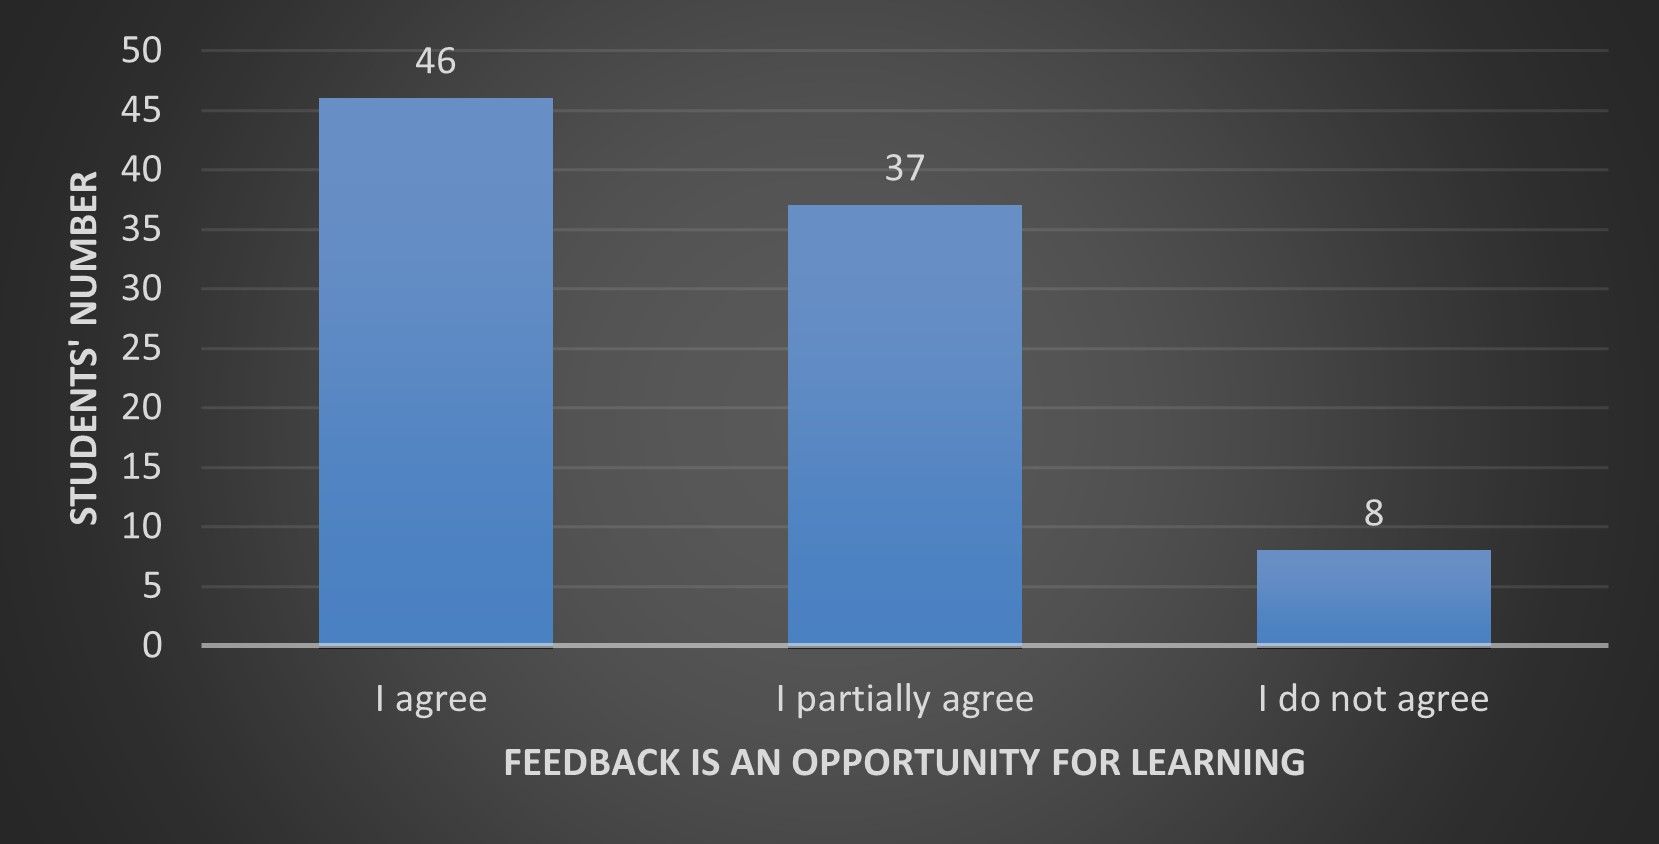
\includegraphics[width=\textwidth]{14.jpg}
 \caption{Perception of oral feedback in virtual classes(a).}
 \label{fig14}
 \source{Own elaboration.}
 \end{minipage}
\end{figure}

The second part of the question clarified the views of students with negative or undecided attitudes. Seven students thought it was embarrassing and demotivating, 50 did not see it as a source of embarrassment, and 34 thought it was embarrassing to a certain extent. Four students did not answer (\Cref{tbl15}, \Cref{fig15}).

\begin{table}[h!]
\centering
\begin{threeparttable}
\caption{Perception of oral feedback in virtual classes(b).}
\label{tbl15}
\begin{tabular}{p{0.3\textwidth} c c}
\toprule
Feedback is embarrassing & Number of students & Percentage \% \\ \midrule
I agree & 7 & 7.69 \\
I partially agree & 34 & 37.36 \\
I do not agree & 50 & 54.94 \\
Total & 91 & 100 \\
\bottomrule
\end{tabular}
\source{Own elaboration.}
\end{threeparttable}
\end{table}

\begin{figure}[h!]
 \centering
 \begin{minipage}{.85\textwidth}
 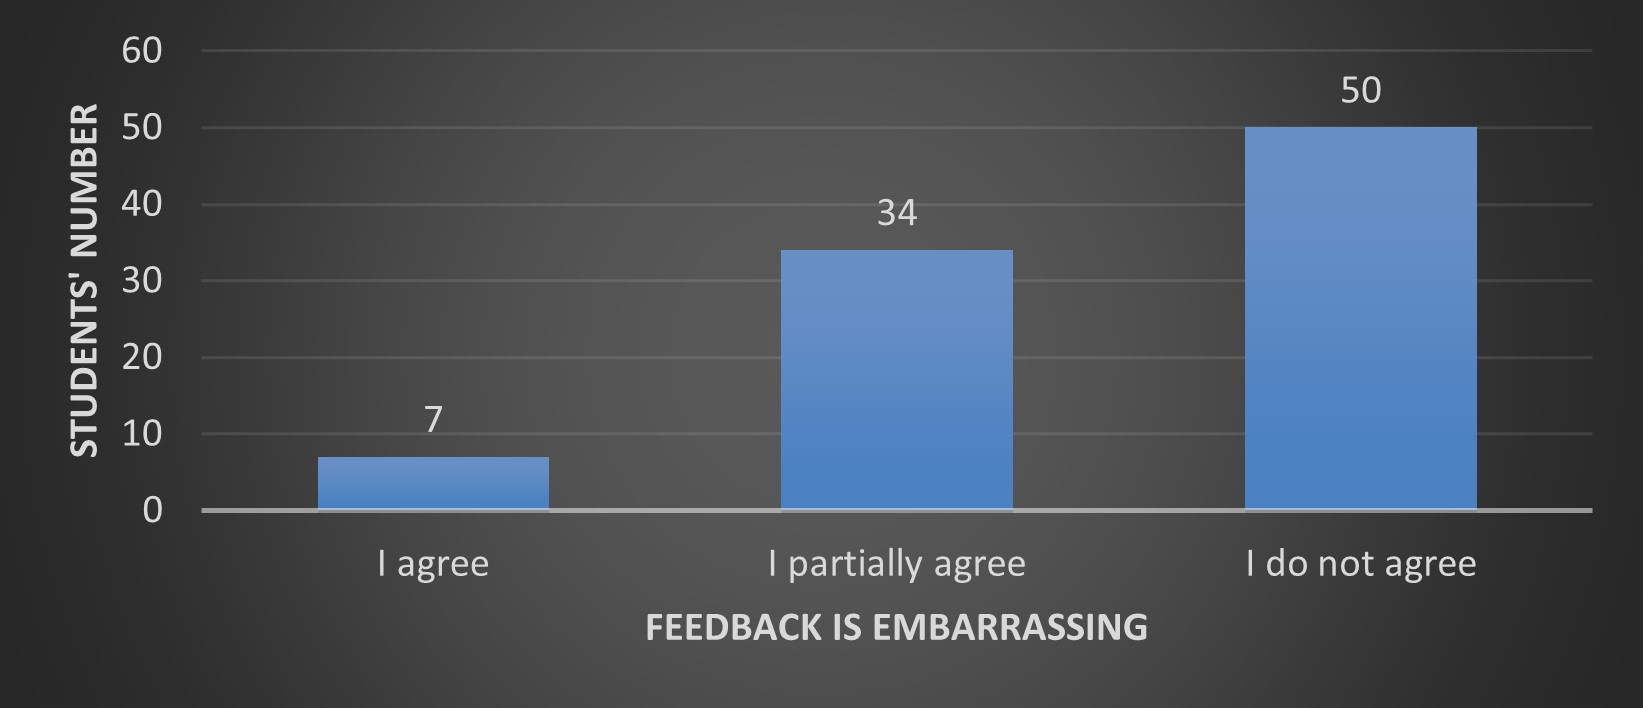
\includegraphics[width=\textwidth]{15.jpg}
 \caption{Perception of oral feedback in virtual classes (b).}
 \label{fig15}
 \source{Own elaboration.}
 \end{minipage}
\end{figure}

Consequently, we had three categories of students: those who appreciated oral feedback in front of their classmates and did not see it as a source of embarrassment, those who had a negative view because they saw it as demotivating, and finally, those who did not take a clear position. They probably recognized its benefit but were not comfortable with the mode, which implies other modes of feedback are potentially more suitable for their psychological needs. To better understand students’ perceptions of feedback that is more suitable to their needs, we asked further questions on their preferences about the way the feedback should take place.

\subsubsection{Preferred delivery mode}

Forty-nine students preferred immediate oral feedback, possibly because it was provided promptly and therefore was more effective. As such, it might help them understand specific aspects of their performance and ways to remediate immediately. Forty-one participants preferred the written mode given privately. They either considered written comments more indelible, providing more opportunities for understanding, or appreciated the private mode because it reduces embarrassment. \textcite[p. 165]{lee_feedback_2018} reported that written comments create good communication and learners view them positively, while \textcite[p. 1508]{ryan_feedback_2019} argued that feedback recorded digitally could be “a promising alternative to both face-to-face dialogue and text-based comments” because it is detailed and indelible at the same time (\Cref{tbl16}, \Cref{fig16}). 

\begin{table}[h!]
\centering
\begin{threeparttable}
\caption{Preferred Delivery Mode.}
\label{tbl16}
\begin{tabular}{p{0.4\textwidth} c c}
\toprule
 & Number of students & Percentage \% \\ \midrule
Oral immediate feedback in front of classmates & 49 & 54.44 \\
Written feedback, given privately & 41 & 45.55 \\
Total & 90 & 100 \\
\bottomrule
\end{tabular}
\source{Own elaboration.}
\end{threeparttable}
\end{table}

\begin{figure}[h!]
 \centering
 \begin{minipage}{.85\textwidth}
 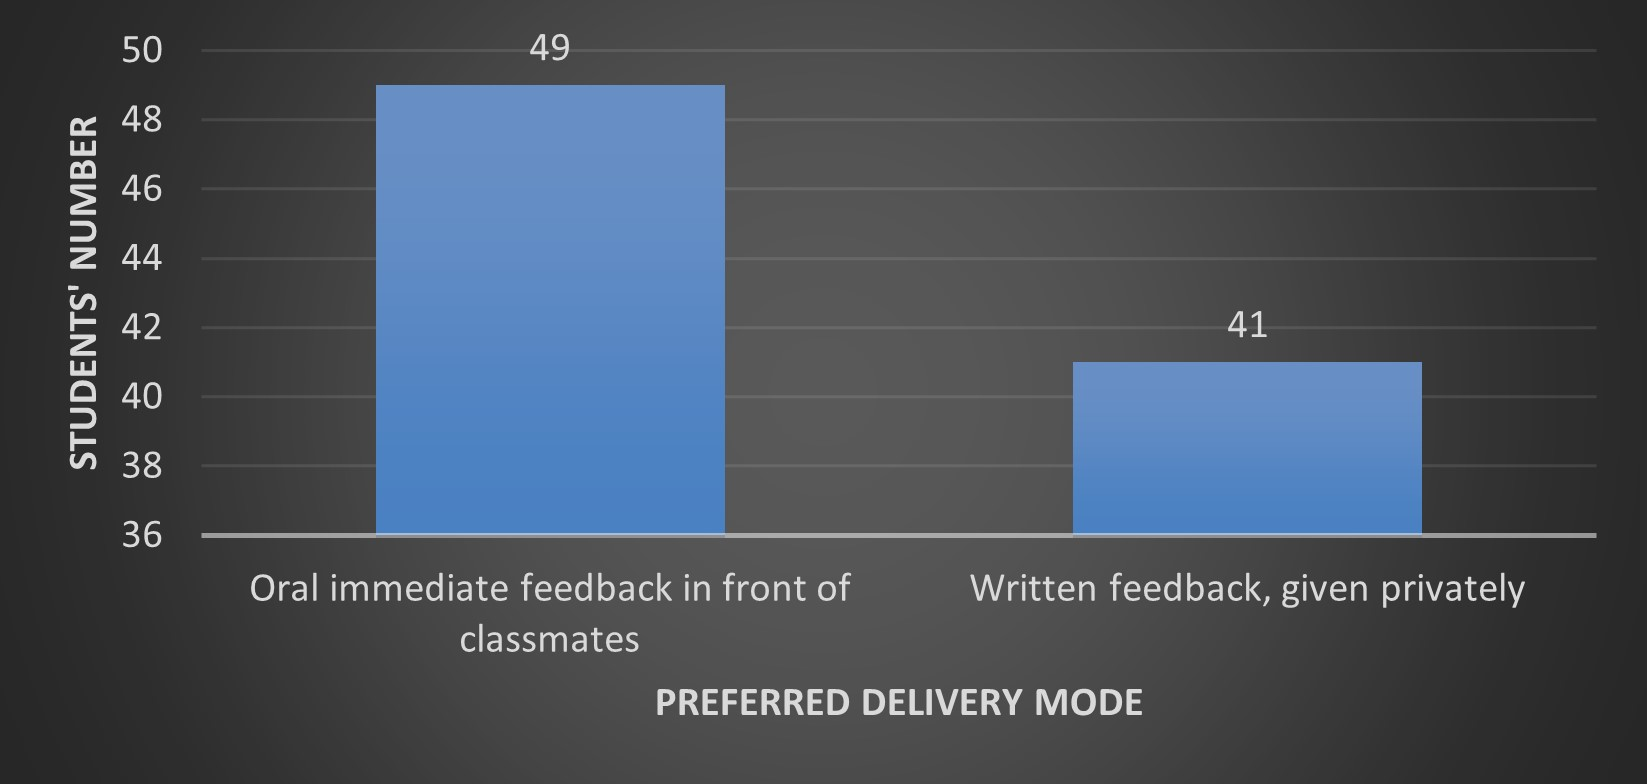
\includegraphics[width=\textwidth]{16.jpg}
 \caption{Preferred Delivery Mode.}
 \label{fig16}
 \source{Own elaboration.}
 \end{minipage}
\end{figure}

\subsubsection{Feedback as a one way or two-way process}

Sixty-six students consider feedback as a process based on a dialogue between the teacher and the student. Twenty-five perceive feedback as comments given by the teacher. Four did not answer the question (\Cref{tbl17}, \Cref{fig17}).

\begin{table}[h!]
\centering
\begin{threeparttable}
\caption{Feedback as a dialogue or as comments.}
\label{tbl17}
\begin{tabular}{p{0.6\textwidth} c c}
\toprule
 & Percentage \% \\ \midrule
A dialogue between teacher and student & 66 & 72.52 \\
Comments from the teacher not requiring any response from the student & 25 & 27.47 \\
Total & 91 & 100 \\
\bottomrule
\end{tabular}
\source{Own elaboration.}
\end{threeparttable}
\end{table}

\begin{figure}[h!]
 \centering
 \begin{minipage}{.85\textwidth}
 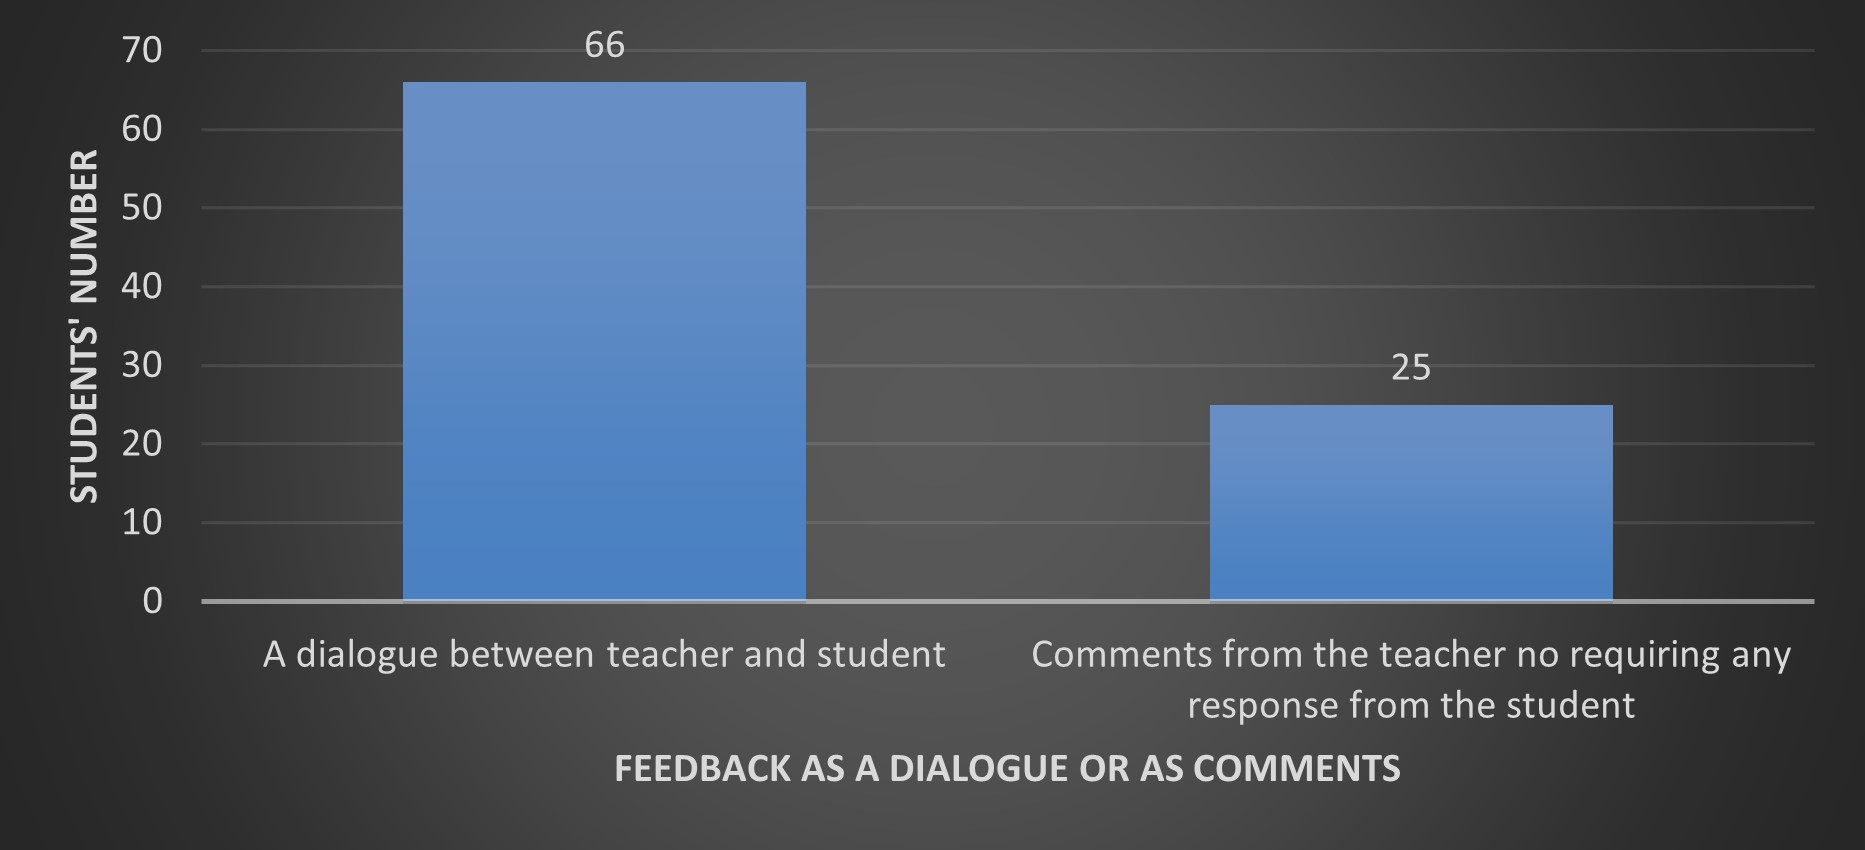
\includegraphics[width=\textwidth]{17.jpg}
 \caption{Feedback as a dialogue or as comments.}
 \label{fig17}
 \source{Own elaboration.}
 \end{minipage}
\end{figure}

The first category of students explained that dialogue is beneficial. It is a method of communication that ensures equality, mutual respect, and cooperation in the classroom. It is advantageous for both parties as it enables the teacher to understand students’ needs and students to better understand their mistakes. It allows them to clarify the points in question and discuss an improvement plan. It is also believed to impact memory positively: through dialogue, information is delivered effectively by the teacher, then memorized by the student.

\begin{quote}
    If there is a dialogue between the student and the teacher, she will not forget this dialogue, but if she receives instructions from the teacher, she will forget this comment.
    
Furthermore, it reduces the feeling of belittlement and enables the student to promote self-confidence:

The teacher should listen to the student's point of view and not give orders without the student's reaction.

Misunderstandings have a greater chance during online classes. Therefore, a dialogue is needed.

Give and take is more fruitful.
\end{quote}

\textcite[p. 6]{torres_interpreting_2016}, recommend that feedback is made as “a personal conversation that remains sensitive to the immediate personal effects on students” because it affects their identities. The second category of students states that dialogue is not required:

\begin{quote}
    When I make a mistake I usually know [..] so the teacher’s feedback will only let me focus on it because
    
I wasn't aware and her telling me about it will help me to focus again. So, I prefer not to respond except if I need an explanation.

Giving Comments on mistakes in front of students helps them learn and this is what is needed.
\end{quote}

Another student commented that she prefers written feedback, while some students explained that it depends on the point:

\begin{quote}
    If I need to talk about it, then dialogue would be suitable, and if not, then teacher comments would be good too.
    
It depends on the comment: some comments require discussion when the student is not convinced and/or feels the need to express her opinion; explain her choice, or when she needs clarifications and arguments from the teacher to understand.
\end{quote}

When asked about how they expect this dialogue to be, they commented that it should cover both areas of strengths and improvement, explain the errors, provide reasons behind term choices, suggest how to correct mistakes, and include a strategy for improvement and advice on effective training:

\begin{quote}
    It should include students’ explanations of choices and point of view.
    
A conversation between two adults who try as hard as they can to deliver information respectfully. And try to understand each other’s point of view. Attentive listening from both parties.

Clear and comprehensible, spontaneous, brief and concise, constructive, includes guidelines and praise

A conversation that leads the students at the end to self-correction.

The teacher should confirm that comments are understood by the student and request an example.

Take into consideration the level and abilities of every student.

All the students benefit from listening to the whole conversation.
\end{quote}

The results of the questionnaire analysis presented above yield key findings that are presented in the next section.

\subsection{Summary of findings}

In accordance with the research questions, our findings can be summarized as follows:

\textbf{Students’ preferences on the mode of feedback}:

Findings indicate that students have different preferences and expectations of feedback. This confirms the findings of other researchers like \cite[p. 156]{lee_feedback_2018} and \cite[p. 325]{odonovan_what_2021}. Several students prefer classroom-based teaching and feedback because they value face-to-face contact and interaction as ensuring more clarity and concentration. Others prefer the distance mode since they believe it is as efficient as the conventional mode or consider online feedback more suitable for their psychological and emotional needs.  However, some believe that feedback efficiency is not dependent on the mode. Delivering information effectively, dedicating enough time to every student, and creating a stimulating environment, are factors that they consider essential.

\textbf{Students’ perceptions of good feedback}:

What is perceived by students as good feedback, whether given onsite or online, is clear, usable, actionable, specific, detailed, non-judgmental feedback given on time \cite[p. 45]{omer_criteria_2017}; \cite[p. 1408]{henderson_conditions_2019}. According to \textcite[p. 322]{odonovan_what_2021}, learners wish to receive “detailed and specific” feedback, indicating that instructors devote time to correct their works. In interpreting classes, students appreciate this kind of feedback because it reflects the teacher’s interest in their performance. Also, good feedback recognizes students’ efforts and, according to \textcite[p. 10]{torres_interpreting_2016}, takes the form of a “personalized” dialogue adapted to the needs of specific situations. It is worth mentioning that students’ preferences and needs emerging from this study and mentioned above should be taken into consideration at the level of teaching, learning and feedback to achieve successful educational processes.

\textbf{Feasibility of using the distance mode}:

Based on students’ answers and comments in open-ended questions, it is more feasible to teach sight interpreting online than bilateral interpreting. Students stated they face more challenges in the latter: it is harder to remember the sentences and ideas included, whereas in the former, the visual aid, i.e., the text shown on the screen, helps them somehow by not wholly relying on memory. Similarly, \textcite{ko_teaching_2009} has conducted a study where he attempted to teach many types of interpreting by using “sound-only teleconference.” This was “feasible both technologically and pedagogically”, and students could attain nearly the same level of onsite students \cite[p. 837-838]{ko_teaching_2009}.

Regarding the skills, paralinguistic skills are the most difficult to address in virtual settings. Because the lectures were conducted without video, the teachers could provide feedback on features based on voice, like intonation and public speaking, but not on other aspects like body language. Our findings are consistent with \textcite[p. 832]{ko_teaching_2009}, who concluded that teaching and monitoring paralinguistic skills “associated with visual interaction” in the distance mode were challenging. They include body language and eye contact, which are not possible to see and assess.  

\subsection{Recommendations}

Based on the research findings, we recommend the following:

1) Using a blended model for training and feedback:

Students’ preferences demonstrate that some prefer the onsite mode, and others prefer the online one. For this reason, we think that a blended model could satisfy the needs of all learners; \textcite[p. 1507]{ryan_feedback_2019} indicate that “it is important to consider the strengths and weaknesses of particular modes, and the value of offering multiple modes.” The technological turn is necessary for the field of training would-be interpreters within a hybrid framework.  Virtual educational environments offer more flexibility because they are not “limited by space and time” \cite[p. 9]{susilana_studentsa_2020}, and providing feedback throughout digital tools could have various benefits for student interpreters \cite[p. 156]{lee_feedback_2018}. For example, \textcite[p. 647]{ahmad_exploring_2021}, where an online flipped class was used to teach English grammar, revealed “the potential” of this learning mode for better students’ achievement.

According to \textcite[p. 39]{kim_flipped_2017}, several empirical studies revealed that blended learning, including the flipped model, is more efficient than both conventional learning and online learning. He himself compared two traditional classrooms with two flipped ones. His study revealed the feasibility of flipped teaching in interpreter training, where conventional instruction is provided through digital platforms while on-campus time is dedicated to interactional activities requiring higher cognitive processes. The benefit is a learner-oriented environment leading to better opportunities for learning \cite[p. 38-39]{kim_flipped_2017}. Moreover, the satisfaction of students and trainers on ORCIT resources created for blended training in postgraduate interpreting programs \cite[p. 3]{carsten_challenge_2021} is another excellent example of the effectiveness of blended models.  

In a study with 4514 students, \textcite[p. 1519]{ryan_feedback_2019} discovered the great benefit of using various feedback modes, “especially if electronic annotations or digital recordings are included”. Also, in the study of \textcite[p. 1410]{henderson_conditions_2019}, a mixture of resources was used to provide feedback to learners: audio recordings and Twitter for text comments. They concluded that they “can complement each other and help learners’ sense-making of the information”.

2) Introducing Remote interpreting courses:

To enable students to understand online feedback and enhance learning and interaction, remote interpreting should be introduced as an independent course in the curriculum \cite[p. 8-11]{karaban_exploring_2021} by elaborating syllabi and disseminating manuals for using CAI tools, i.e., computer-assisted interpreting tools.

3) Several things matter to make feedback effective.
Research indicates that several factors contribute together to make feedback good.  

Generally good feedback, whether onsite or online, is the one that makes a balance between the two sides described by \textcite[p. 811]{leighton_students_2019}: the external (instructionally relevant) and internal (psychologically relevant) sides “to get the learning right not just for behavioral outcomes but for cognitive and emotional ones too”.

4) Developing feedback literacy among students:

Students who do not acknowledge the function and importance of feedback in learning, and are not aware of their responsibility in using it for future improvement, will be unable to understand teacher feedback and act upon it. Therefore, it is necessary to develop this ability among them. Using \posscite{carless_development_2018} Framework of feedback literacy, including appreciating feedback; making judgments; managing affect; and taking action, we suggest the following steps to develop feedback literacy among students in interpreting classrooms, whether onsite, online or within a blended setting:

Stage one - Introducing the notions of feedback, interpreting quality, and assessment criteria to students:

At the beginning of the term, the teacher talks about feedback explicitly: he/she explains the concept of feedback, its value, and the role of the teacher and the learner in the feedback process, as well as the notion of quality in interpreting, by explaining the criteria used in the rubrics for assessing interpretations in projects and exams. It is not sufficient to send the rubrics on learning management systems or discuss them incidentally. According to \textcite[p.1322]{carless_development_2018}, “meta-dialogues discuss processes and strategies of assessment and feedback rather than the specifics of a particular piece of work”. These meta-dialogues are necessary to raise students’ awareness about the nature of the feedback process, and then they will gradually appreciate it and fully take part in it.
Stage two- Developing students’ capacity in self and peer-assessment to understand teacher feedback:

By creating a safe learning environment and providing guidance, the teacher creates opportunities for students to participate actively in peer and self-feedback activities. It may start -using the words of \textcite[p. 1321]{carless_development_2018} - by “showing them rather than telling them about quality work”. We suggest offering them examples of good interpretations as they conduct sight and bilateral interpreting activities. This modeling by the teacher and the student-generated feedback should be enhanced with explicit criteria introduced in the first stage to build critical thinking skills. Furthermore, during these activities, the teacher should offer guidance and advice on managing negative emotions that may be triggered in feedback settings. All these activities can be conducted in face-to-face classrooms or moved online using Blackboard, Zoom, social media platforms, audio and video recordings… etc.

Stage three- Students act on feedback and give evidence on that:
For feedback to have any benefit and value, learners should take action by using teacher comments in their subsequent assignments. \textcite[p. 11]{hoo_developing_2022} stress the importance of making plans to achieve specific goals, determining actions required to implement those plans, and “monitoring progress.” This will enhance “self-accountability” among students and enable them to “close the loop of learning from feedback”. Similarly, we suggest “closing the feedback loop” \cite[p. 1323]{carless_development_2018} and \cite[p. 11]{hoo_developing_2022} in the interpreting classroom, viewing feedback as a “cycle” \cite{van_de_ridder_what_2008} and feedback processes as including “multiple cycles” \cite[p  47]{omer_criteria_2017}. Conversations should be held in different settings where students are continuously required to demonstrate how they have used teacher feedback to improve their performance. The \Cref{fig18} summarizes the stages we suggest for building students’ capacity to understand better, use, and take benefit from feedback.

\begin{figure}[h!]
 \centering
 \begin{minipage}{.85\textwidth}
 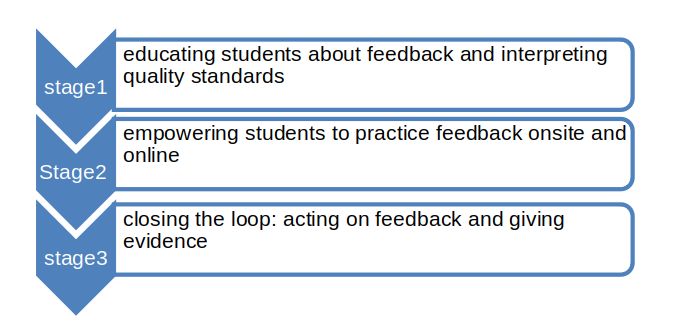
\includegraphics[width=\textwidth]{18.png}
 \caption{Feedback cycle in interpreting classrooms.}
 \label{fig18}
 \source{Own elaboration.}
 \end{minipage}
\end{figure}


\section{Conclusion}\label{sec-formato}
This study investigated students’ perceptions of teacher feedback in the sight and bilateral interpreting classroom. The questionnaire-based survey conducted with 95 undergraduate female students explored issues related to the effectiveness of online feedback at the cognitive and emotional levels as well as the challenges it implies and students’ expectations. Findings indicate that students have conflicting views and preferences on online feedback.

The study recommends teaching remote interpreting, considering the different factors affecting the feedback process, and developing students’ capacity to understand and act on feedback in the interpreting classroom by following different steps. This will help to reconcile teachers’ beliefs and students’ expectations about ‘good feedback’. The best lesson learned from this study is that online teaching and feedback are valuable and satisfy the emotional needs of some students. For this reason, we suggest using a blended model for teaching interpreting and providing digital feedback using different platforms in the near future.

Further research needs to explore the efficiency of online tools and methods for teaching courses of “remote interpreting” as an independent discipline as well as blended interpreting and translation courses and investigate new ways for reinforcing feedback usability among students, especially online and digital feedback.

\printbibliography\label{sec-bib}
% if the text is not in Portuguese, it might be necessary to use the code below instead to print the correct ABNT abbreviations [s.n.], [s.l.]
%\begin{portuguese}
%\printbibliography[title={Bibliography}]
%\end{portuguese}



\end{document}

